\documentclass[14pt,a4paper]{scrartcl}
\usepackage[utf8]{inputenc}
\usepackage{ragged2e}
\usepackage{mathtools}
% \usepackage{esint}
\usepackage[english,russian, ukrainian]{babel}
\usepackage{misccorr,color,ragged2e,amsfonts,amsthm,graphicx,systeme,amsmath,mdframed,lipsum}
\renewcommand\qedsymbol{$\blacksquare$}
\renewcommand*{\proofname}{\text{Доведення}}
\theoremstyle{definition}
\newtheorem*{defo}{Означення}
\newtheorem*{teo}{Теорема}
\newtheorem*{example}{Приклад}
\theoremstyle{remark}
\newtheorem*{remark}{Зауваження}
\theoremstyle{definition}
\newtheorem*{consequence}{Наслідок}
\theoremstyle{definition}
\newtheorem{statement}{Утверждение}[section]
\newmdtheoremenv{boxteo}{Теорема}[section]
\setlength\parindent{0pt}
\DeclareMathOperator*\lowlim{\underline{lim}}
\DeclareMathOperator*\uplim{\overline{lim}}
\newcommand\independent{\protect\mathpalette{\protect\independenT}{\perp}}
\def\independenT#1#2{\mathrel{\rlap{$#1#2$}\mkern2mu{#1#2}}}
%
% \makeatletter
% %% make esint definition in line with amsmath
% \@for\next:={int,iint,iiint,iiiint,dotsint,oint,oiint,sqint,sqiint,
%   ointctrclockwise,ointclockwise,varointclockwise,varointctrclockwise,
%   fint,varoiint,landupint,landdownint}\do{%
%     \expandafter\edef\csname\next\endcsname{%
%       \noexpand\DOTSI
%       \expandafter\noexpand\csname\next op\endcsname
%       \noexpand\ilimits@
%     }%
%   }
% \makeatother
% Default fixed font does not support bold face
\DeclareFixedFont{\ttb}{T1}{txtt}{bx}{n}{12} % for bold
\DeclareFixedFont{\ttm}{T1}{txtt}{m}{n}{12}  % for normal

% Custom colors
\usepackage{color}
\definecolor{deepblue}{rgb}{0,0,0.5}
\definecolor{deepred}{rgb}{0.6,0,0}
\definecolor{deepgreen}{rgb}{0,0.5,0}

\usepackage{listings}

% Python style for highlighting
\newcommand\pythonstyle{\lstset{
language=Python,
basicstyle=\ttm,
otherkeywords={self},             % Add keywords here
keywordstyle=\ttb\color{deepblue},
emph={MyClass,__init__},          % Custom highlighting
emphstyle=\ttb\color{deepred},    % Custom highlighting style
stringstyle=\color{deepgreen},
frame=tb,                         % Any extra options here
showstringspaces=false            %
}}

\definecolor{javared}{rgb}{0.6,0,0} % for strings
\definecolor{javagreen}{rgb}{0.25,0.5,0.35} % comments
\definecolor{javapurple}{rgb}{0.5,0,0.35} % keywords
\definecolor{javadocblue}{rgb}{0.25,0.35,0.75} % javadoc

\lstset{language=C++,
basicstyle=\ttfamily,
keywordstyle=\color{javapurple}\bfseries,
stringstyle=\color{javared},
commentstyle=\color{javagreen},
morecomment=[s][\color{javadocblue}]{/**}{*/},
numbers=left,
numberstyle=\tiny\color{black},
stepnumber=2,
numbersep=10pt,
tabsize=4,
showspaces=false,
showstringspaces=false}


% Python environment
\lstnewenvironment{python}[1][]
{
\pythonstyle
\lstset{#1}
}
{}

% Python for external files
\newcommand\pythonexternal[2][]{{
\pythonstyle
\lstinputlisting[#1]{#2}}}

% Python for inline
\newcommand\pythoninline[1]{{\pythonstyle\lstinline!#1!}}
%
% \begin{python}
% class MyClass(Yourclass):
%     def __init__(self, my, yours):
%         bla = '5 1 2 3 4'
%         print bla
% \end{python}

\begin{document}



\def\be{\begin{equation}}
\def\ee{\end{equation}}
\def\bd{\begin{defo}}
\def\ed{\end{defo}}
\def\bbt{\begin{boxteo}}
\def\ebt{\end{boxteo}}
\def\i{\infty}
\def\d{\partial}

\begin{center}
	\Huge \textbf{Собственно, теорвер...}
\end{center}

\tableofcontents

\pagebreak




\section{Абсолютно неперервні розподіли.}

\subsection{Рівномірний розподіл.}

Рівномірний розподіл на $[a,b]$. Графік функції щільності розподілу:\\
\begin{center} 
\includegraphics[scale=0.3]{images/2.png} \end{center}
Позначення: $\xi \sim U(a,b)$. Функція щільності має наступній вигляд:\\
$$
f_\xi (x) = \left\lbrace \begin{gathered}
 c, x \in [a,b] \\
 0, x \notin [a,b]
 \end{gathered} \right. , \text{ де } c = \frac{1}{b-a}
$$
Визначимо функцію розподілу: $$F_\xi (x) = \left\lbrace
\begin{gathered}
0, x \in (-\infty; a]\\
	\int\limits_{a}^{ t}{f_\xi (t) dt} = \frac{1}{b-a} x - \frac{a}{a-b}  = \frac{x-a}{b-a}, x \in (a,b] \\
1, x \in (b; + \infty)
\end{gathered} \right.   $$
Числові характеристики:\\
$ \mathbb{E} \xi  =   \int\limits_{a}^{ b}{ x  f_\xi (x) dx} = \frac{b^2 - a^2}{2b - a}  = \frac{a+b}{2} $ \\
$ \mathbb{E} \xi^2 =  \int\limits_{a}^{ b}{x^2 f_\xi (x) dx} = \frac{1}{b-a} \frac{x^3}{3} \Big|_a^b = \frac{b^3 - a^3}{3(b-a)} = \frac{a^2 + ab + b^2}{3}   $\\
$ \mathbb{D} \xi =  \frac{a^2 + ab + b^2}{3} - \frac{a^2 + 2ab + b^2}{ 4} = \frac{(a-b)^2}{12}  $\\
Величини залежать лише від довжини проміжку.\\ Нехай $[c,b] \subset [a,b]$, тоді знайдемо:
$$
\mathbb{P} \left\lbrace \xi \in [c,d] \right\rbrace = F_\xi(d) - F_\xi (c) = \frac{d-c}{b-a}
$$
\subsection{Експоненціальний розподіл.}
Розглядаємо $ \xi \sim Exp(\lambda), \lambda > 0$. \\
Щільність розподілу:
$$
f_\xi (x) =
 \left\lbrace \begin{gathered} \lambda e^{-\lambda x}, x \geq 0 \\
 0 , x <0 \end{gathered}
 \right.
 \qquad \qquad
 \begin{gathered}
 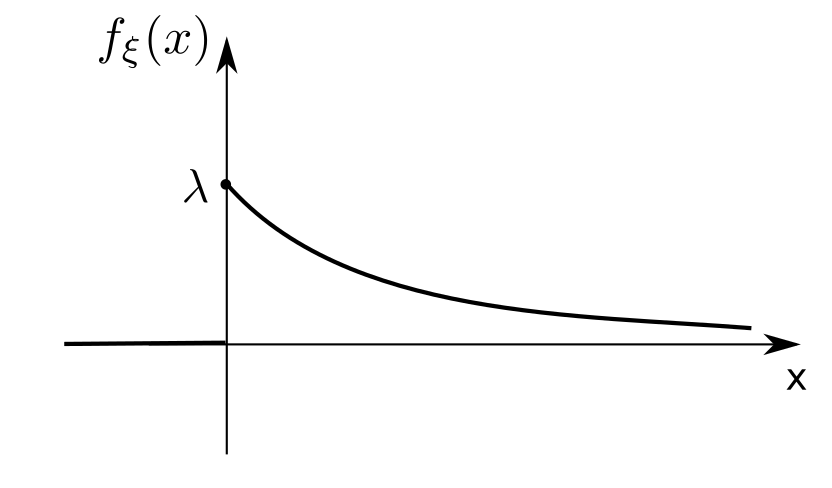
\includegraphics[scale=0.25]{images/3.png}
 \end{gathered}
$$
Запишемо функію розподілу:
$$
F_\xi (x) = \left\lbrace
\begin{gathered}
  \int\limits_{-\infty}^{ x}{ 0 dt} = 0,\qquad x < 0\\
	F(0)+  \int\limits_{0}^{x}{ \lambda e^ {-\lambda t} dt} = 1 - e^ {- \lambda x}, x \geq 0
\end{gathered} \right. \begin{gathered} 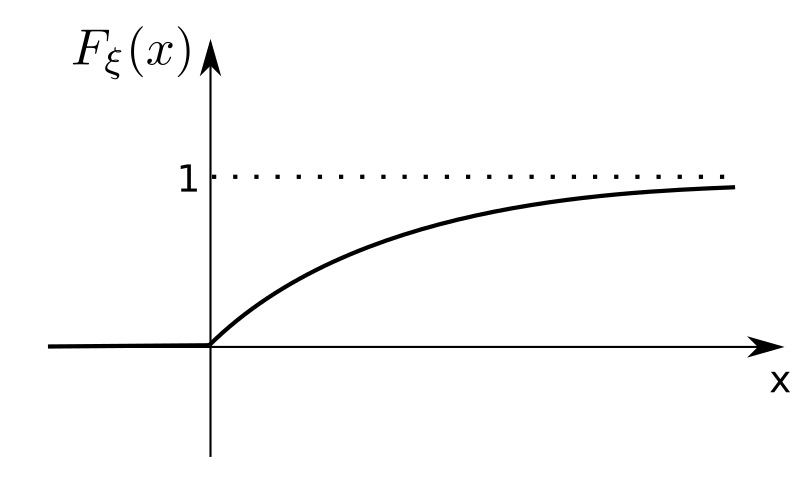
\includegraphics[scale=0.25]{images/1.png}
\end{gathered}
$$
Знайдемо: $ \mathbb{P} \left\lbrace \xi \in [x,d] \right\rbrace  = (1 - e^ { - \lambda x})\Big|^d_c = e^{- \lambda c} - e^{- \lambda d}$.\\
Виведемо числові характеристики. Спочатку виведемо формулу $ \forall k \in \mathbb{N}: \mathbb{E} \xi^k:$
$$
 \int\limits_{- \infty}^{ +\infty}{ x^k * f_\xi (x) dx} = \lambda \int\limits_{- \infty}^{ +\infty}{ x^k e^{ - \lambda x} dx} = \frac{1}{ \lambda^k}  * \text{Г}(k+1) = \frac{k!}{\lambda^k}
$$
Користуючись цією формулою, отримаємо числові характеристики розподілу:

$$
\begin{gathered}
 \mathbb{E} \xi = (k=1) = \frac{1}{\lambda} \\
 \mathbb{E} \xi^2 = (k=2) = \frac{2}{\lambda^2} \\
 \mathbb{D} \xi =  \frac{2}{\lambda^2}  - \frac{1}{\lambda^2} = \frac{1}{\lambda^2}  \\
\end{gathered}
\qquad \qquad\qquad\qquad\qquad
\left|
\begin{gathered}
\textbf{Властивості Гамма-функції: }\\
 1. \text{Г}(\alpha) =  \int\limits_{0}^{ \infty}{ x^{\alpha -1 } e^{-x} dx}\\
 2. \text{Г} (n) = (n-1)!\\
 3. \text{Г} (\alpha+1) = \alpha * \text{Г}(\alpha)\\
 4. \text{Г} (1/2) = \sqrt{\pi}
\end{gathered}
\right|
$$

\begin{center}
	Експоненціальна величина описує час безвідмовної роботи приладу до моменту першої відмови. Це твердження не є вірним. Чому?
\end{center}

\textbf{Властивості експоненціального розподілу.}\\
1. Відсутність післядії. \\
$$ \xi \sim Exp(\lambda) \Rightarrow  \begin{gathered}
 \forall t, h > 0 \\
 \mathbb{P} \{ \xi > t+h \big| \xi >t \}  = \mathbb{P} \{ \xi > h \}
\end{gathered}
$$

\begin{proof}
$$
 \mathbb{P} \{ \xi > t+h \big| \xi >t \}  = \frac{ \mathbb{P} \{ \xi > t+h, \xi > t \}}{ \mathbb{P} \{ \xi > t \}} =
  \frac{ \mathbb{P} \{ \xi > t+h \}}{\mathbb{P} \{ \xi > t \} }=
 \frac{ e^{-\lambda (t+h) - e^{-\lambda \infty}} }{ e^{- \lambda t} - e^ {-\lambda \infty} } =
 $$
$$
= e^{-\lambda h} - e^{-\lambda\infty } = \mathbb{P} \left\lbrace \xi  > h \right\rbrace
$$
\end{proof}

2. Стійкість відносно min.\\
$ \xi_1, \xi_2 ... , \xi_n$ - незалежні.$ \left(  \begin{gathered}
\xi_1 \sim Exp(\lambda_1) \\
 \xi_2 \sim Exp(\lambda_2) \\
 ...\\
 \xi_n \sim Exp(\lambda_n) \\
\end{gathered} \right) $  $ \Rightarrow \min \left\lbrace  \xi_1 , \xi_2, .,. , \xi_n \right\rbrace  \sim Exp (  \sum\limits_{i = 1}^{ n}{ \lambda_i})$
\begin{proof}

$$
F_{min(\xi_1, ..., \xi_n)} (x) = \mathbb{P} \left\lbrace \min \left(\xi_1, ... , \xi_n  \right) < x  \right\rbrace  = 1 - \mathbb{P} \left\lbrace \min \left(\xi_1, ... , \xi_n  \right) \geq  x  \right\rbrace =
$$
$$
1 - \mathbb{P} \left\lbrace  \xi_1 \geq x, ... , \xi_n \geq x \right\rbrace = 1 - \mathbb{P} \left\lbrace \xi_1 \geq  x \right\rbrace \cdot ... \cdot \mathbb{P} \left\lbrace   \xi_n \geq 1\right\rbrace = 1 - e ^ { - \lambda_1 x} \cdot e^ { -\lambda_2 x} \cdot ... \cdot e^{- \lambda_n x} =
$$
$$
 = F_{Exp(\lambda_1 + \lambda_2 + ... + \lambda_n)} (x), x\geq 0
$$

\end{proof}
Використання: нехай є прилад, що складається з $n$ блоків. Для коректної роботи приладу необхідно коректна робота всіх блоків. \\
Позначимо: $\xi_i$ - час роботи блоку $i, i = 1, ..., n$.\\
Час роботи всього приладу: $ \xi = \min \left\lbrace \xi_1, \xi_2, ..., \xi_n \right\rbrace $.
\begin{example}
	Прилад - 10 блоків. Кожний з них з ймовірністю 0.99 може пропрацювати 1000 годин. Знайти середній час роботи всього приладу та ймовірність того, що він пропрацює 500 год.\\
	Розглянемо блок і-тий: \\$ \xi_i = Exp(\lambda_i)$.\\
	$\mathbb{P} \left\lbrace \xi_i \geq 1000 \right\rbrace = 0.99 = e ^ {-1000 \lambda} \Longrightarrow \lambda = \frac{ \ln{0.99}}{-1000} \approx 10^{-5}$\\
	$\mathbb{E} \xi_i = \frac{1}{\lambda} = 10^5 $\\
	Для всього приладу:\\
	$ \xi = \min \left\lbrace \xi_1, ... , \xi_n \right\rbrace  \sim Exp( \sum\limits_{i = 1}^{ 10}{\lambda_i}) = Exp(10^{-4})$\\
	$ \mathbb{E}\xi = 10^4 \qquad \mathbb{P} \left\lbrace \xi \geq 500 \right\rbrace = e^{-500 * 10^{-4}} = e^{-0.005} \approx 0.95$
\end{example}
3. Inter-arrival times dependency.
\begin{boxteo}
Розглянемо потік Пуассона з інтенсивністю
 $$\lambda \Rightarrow  N(s,t) \sim Pois(\lambda(t-s)) $$
\begin{center} 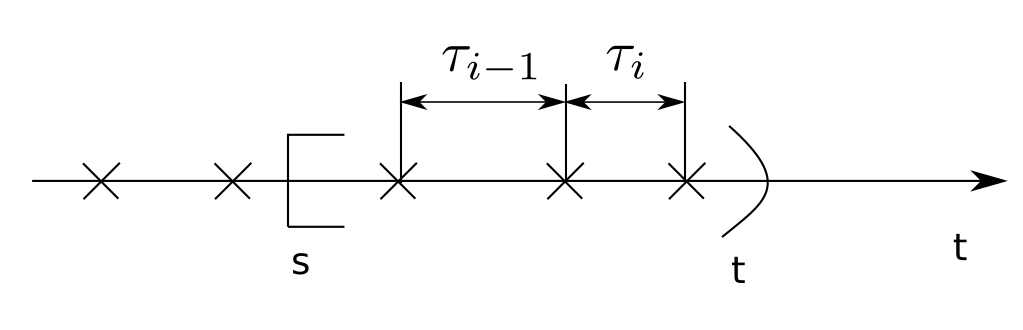
\includegraphics[scale=0.3]{images/4.png} \end{center}
$\tau_i - $ inter-arrival times.
 $ \Rightarrow\left( \tau_i , i \in \mathbb{Z} \right) - $ незалежні, та $Exp(\lambda).$
\end{boxteo}
\subsection{ Гаусівський (нормальний) розподіл.}
\textbf{Стандартний Гаусівський розподіл.} Позначення:
$$
\xi \sim N (0, 1^2)
$$
Щільність розподілу:
$
f_{\xi} (x) = C \cdot e^{- \frac{x^2}{2} }
$.
З умови нормування та властивостей Гамма-функції:
$$  1 = \int\limits_{- \infty}^{ +\infty}{ f_ \xi (x) dx} = 2C  \int\limits_{0}^{ \infty}{ e^ { -\frac{x^2}{2} } dx} = \left|  \begin{gathered}
 \frac{x^2}{2} = t  \\
 x = \sqrt{2t} \\
 dx = \frac{dt}{\sqrt{2t}}
\end{gathered} \right|  =  2C  \int\limits_{0}^{ +\infty}{e^{-t} \frac{dt}{\sqrt{2} \cdot \sqrt{t}} } = $$
$$
= \sqrt{2} C  \int\limits_{0}^{\infty}{ t^{-1/2} e^{-t}dt} = \sqrt{2} C \text{Г}(1/2) = \sqrt{2\pi}C \Longrightarrow C = \frac{1}{\sqrt{2\pi}}
$$
$$
\begin{gathered}
\text{Остаточно, }\\
\text{щільність розподілу: }\\
f_ \xi (x) = \frac{1}{ \sqrt{2\pi} } e^{ - \frac{x^2}{2} }, \quad x \in \mathbb{R}
\end{gathered}\qquad\qquad \begin{gathered} 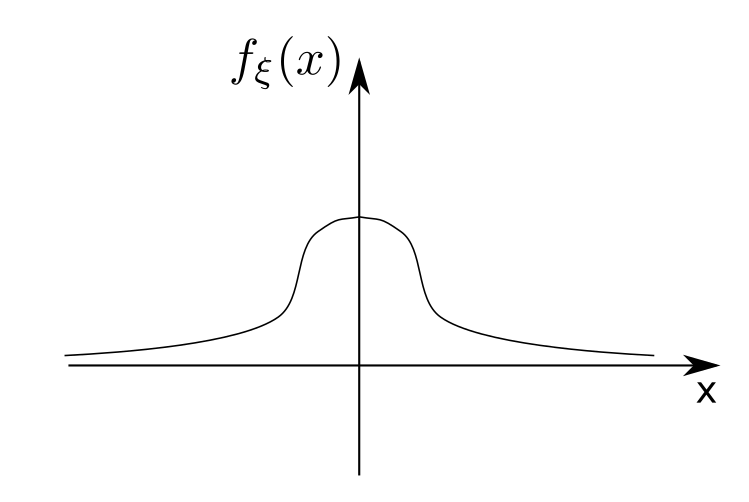
\includegraphics[scale=0.3]{images/5.png} \end{gathered}
$$
Знайдемо числові характеристики розподілу:\\
$ \mathbb{E} \xi =  \int\limits_{- \infty}^{ +\infty}{ x * \frac{1}{ \sqrt{2\pi} } e^{ - \frac{x^2}{2} } dx} = 0$ (Функція щільності парна)\\
$\mathbb{D} \xi = \mathbb{E} \xi^2 =  \int\limits_{- \infty }^{ +\infty}{ x^2 \frac{1}{ \sqrt{2\pi} } e^{ - \frac{x^2}{2} } dx} = \sqrt{\frac{2}{\pi}}  \int\limits_{0}^{\infty}{x^2
e^ {-x^2/2}dx
}  =  \sqrt{\frac{2}{\pi}}  \int\limits_{0}^{\infty}{2t
e^ {-t} \frac{dt}{ \sqrt{2t}}} = \frac{2}{\sqrt{\pi}}  \int\limits_{0}^{\infty}{ t^ {1/2} e^{-t} dt} = \\ = \frac{2}{\sqrt{\pi}} \text{Г}(3/2) = \frac{2}{\sqrt{\pi}} \cdot \frac{1}{2} \cdot \text{Г}( \frac{1}{2} )   = 1  $\\
Для гаусівського розподілу: $N(a, \sigma^2)$, де $a = \mathbb{E} \xi \quad \sigma = \sqrt{\mathbb{D} \xi}$\\
$$
F_ \xi (x) =  \int\limits_{- \infty}^{ x}{ f_ \xi (t) dt} =  \int\limits_{- \infty}^{ x}{ \frac{1}{\sqrt{2\pi}  }e^{ - \frac{t^2}{2}} dt } =  \int\limits_{- \infty}^{0}{\frac{1}{\sqrt{2\pi}  }e^{ - \frac{t^2}{2}} dt } +  \int\limits_{0}^{ x}{\frac{1}{\sqrt{2\pi}  }e^{ - \frac{t^2}{2}} dt } =
 \frac{1}{2} + \Phi(x)
$$
$\Phi (x) = \frac{1}{\sqrt{2\pi}}  \int\limits_{0}^{ x}{ e^{ - \frac{t^2}{2} } dt} $  - функція Лапласа aka \textbf {CDF }(cumulative distr. function).\\
$\xi \sim N(0,1).$ Знайдемо $ \mathbb{P} \left\lbrace \xi \in [b,c] \right\rbrace,\mathbb{E} \xi^k, k \in \mathbb{N}$:
$$
\mathbb{P} \left\lbrace  \xi \in [b,c] \right\rbrace = F_ \xi (c) - F_ \xi( b) = \Phi (c)- \Phi (b)
$$

$$
k = 2n, n\in \mathbb{N} \qquad \mathbb{E} \xi^k =   \int\limits_{0}^{ +\infty}{ x^k e^ { -x^2/2 }dx} = \frac{2^{k/2}}{\sqrt{\pi}}  \int\limits_{0}^{ +\infty}{ t^ { \frac{k-1}{2}  } e^{-t} dt} = \frac{2^ \frac{k}{2} }{ \sqrt(\pi) } \text{Г} ( \frac{k+1}{2} ) =
$$
$$
= \frac{2^ {k/2}}{\sqrt{\pi}} \cdot \frac{k-1}{2} \cdot \frac{k-3}{2}  \cdot ... \cdot \frac{3}{2} \cdot \frac{1}{2} \cdot \text{Г} ( \frac{1}{2} )= \frac{2^{ \frac{k}{2} }}{\sqrt{\pi}}\cdot \frac{(k-1)!!}{ 2^{ \frac{k}{2} }} \cdot \sqrt{\pi} = (k-1)!!
$$
$$
\mathbb{E} \xi ^k =   \int\limits_{-\infty}^{ +\infty}{ x^k \frac{1}{ \sqrt{2 \pi}} e ^ { - \frac{x^2}{2} } dx} = \left\lbrace \begin{gathered}
 (k-1)!! ,\quad k = 2n, n \in \mathbb{N}\\
 0 ,\qquad k = 2n+ 1, n \in \mathbb{N}
\end{gathered} \right.
$$
Перейдемо до загального гаусівського розподілу.\\
\textbf{Загальний гаусівський розподіл.}
\begin{defo}
Візьмемо, що $\xi_0 \sim N(0, 1)$ - стандартна гаусівська величина. \\
$\xi$ називається гаусівською величиною: $ \xi \sim N(a, \sigma^2)$, якщо $ \xi = a + \sigma \xi_0$ - існує та справедливе перетворення стандартної гаусівської величини.
\end{defo}
Числові характеристики гаусівського розподілу:\\
$\mathbb{E} \xi = \mathbb{E}(a + \sigma \xi_0) = a$\\
$\mathbb{D} \xi = \mathbb{D} (a + \sigma \xi) = \sigma^2 \mathbb{D} \xi = \sigma^2$\\
$ F_ \xi (x) = \mathbb{P} \left\lbrace \xi <x \right\rbrace = \mathbb{P} \left\lbrace a + \sigma\xi  < x \right\rbrace = \mathbb{P} \left\lbrace \xi_0 < \frac{x-a}{ \sigma}  \right\rbrace = F_ { \xi_0}( \frac{x-a}{\sigma} 	) = \frac{1}{2} + \Phi ( \frac{x-a}{\sigma} ) $ \\
$\mathbb{P} \left\lbrace  \xi \in [b,c] \right\rbrace = F_ \xi (c) - F_ \xi (b) = \Phi( \frac{c-a}{\sigma} ) - \Phi( \frac{b-a}{\sigma} )$\\

Знаючи $ F_ \xi (x) $  знайдемо вираз для щільності розподілу:
$$
f_ \xi (x ) = F` \xi (x) =  \frac{1}{\sqrt{\pi}} e^{ - (\frac{x-a}{\sigma})^2/2 } \cdot \frac{1}{\sigma}  =  \frac{1}{\sigma \sqrt{2\pi}} e^ { - \frac{(x-a)^2}{2 \sigma^2} }
$$
$$
E_{N(a, \sigma^2)} =  \frac{ \mathbb{E} \left( \xi - \mathbb{E} \xi \right)^4 }{ \left( \mathbb{D} \xi \right)^2 }  -3
 =\left|
\begin{gathered}
 \xi = a \sigma \xi_0 \\
 \mathbb{E} \xi = a
\end{gathered}
 \right|
 = \frac{ \sigma ^4 \mathbb{R} \xi_0^4 }{ \sigma^4} - 3 = \mathbb{E} \xi_0^4 - 3 = 0
$$
\textbf{Правило } $ \mathbf{``3 \sigma``}$. \quad $ \xi \sim (a, \sigma^2)$ \quad Знайдемо:
$\mathbb{P} \left\lbrace  \left| \xi - a \right | < 3 \sigma  \right\rbrace
 = \\ = \mathbb{P} \left\lbrace  \xi \in (a - 3 \sigma; a + 3\sigma) \right\rbrace
= \Phi ( \frac{a + 3\sigma  -a  }{\sigma}  - \Phi( \frac{a - 3\sigma - a}{\sigma} )) = 2\Phi (3) \approx 0.9974
$\\
Тобто, у багатьох практичних випадках, гаусівська величина відповідає нерівності $\left| \xi - a \right | < 3 \sigma$ з великою вірогідністю.\\


\begin{boxteo}[Центральна гранична теорема]
Розглянемо $\xi_1, \xi_2, ... , \xi_n$ - незалежні, мають однаковий розподіл.
Якщо $\mathbb{E} \xi_i = 0 $ та $\mathbb{D} \xi_1 = 1$ :
$$
\frac{\xi_1 + \xi_2 + ... + \xi_n}{\sqrt{n}} \begin{gathered}
 d\\ \longrightarrow \\
 n \to \infty
\end{gathered}  N (0,1)
$$
\end{boxteo}
Гаусівська випадкова величина добре описує результат дії великої кількості випадкових факторів, дія кожного з яких окремо є досить малою.

\section{Випадкові вектори}
Розглядаємо: $$ \vec{ \xi} = \begin{bmatrix}
 \xi_1 \\
 \xi_2\\
 ...\\
 \xi_n
\end{bmatrix}$$

\begin{defo}
	Випадковий вектор - система випадкових величин $ \xi_1 ... \xi_n$, що задані на спільному ймовірністному просторі $ (\Omega, F, \mathbb{P})$.
\end{defo}

Функція розподілу: $ F_{\vec{\xi}} ( x_1, ..., x_n) = \mathbb{P} \left\lbrace \xi_1 < x_1, ..., \xi_n < x_n \right\rbrace$.
$$
\begin{gathered}
\overline{\xi} = \begin{bmatrix}
\xi_1 \\
\xi_2\\
\end{bmatrix}  \\  \\ F_{\overline{\xi}} (x,y) = \mathbb{P} \left\lbrace \xi_1 < x, \xi_2 < y \right\rbrace
\end{gathered} \qquad\qquad\qquad
\begin{gathered}
 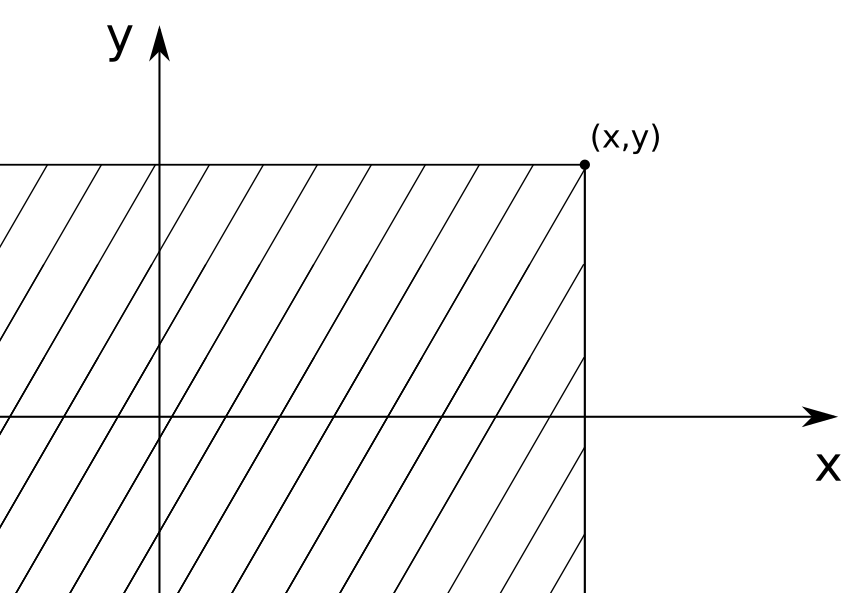
\includegraphics[scale=0.21]{images/9.png}
\end{gathered}
$$
% graphicx
\subsection{Властивості функції  розподілу.}

1. $F_{\overline{\xi}} (x,y) \in [0,1] \quad \forall x,y \in \mathbb{R}$\\
2. $ F_{ \overline{\xi}} $ - неспадна для кожного аргументу. Тобто:
\begin{center}
	$F_{\overline{\xi}} (x_1, y) \leq F_{\overline{\xi}} (x_2, y)$ при $ x_1 \leq x_2$;\\ $ F_{\overline{\xi}} (x, y_1) \leq F_{\overline{\xi}} (x, y_2)$ при $ y_1 \leq y_2$.
\end{center}
$$
\mathbb{P} \left\lbrace \xi_1 < x_1, \xi_2 < y \right\rbrace \leq \mathbb{P} \left\lbrace \xi_1 < x_2, \xi_2 < y \right\rbrace
$$
3, $ F_{\overline{\xi}} $ - неперервна зліва за кожним аргументом. \\
4a.$$
\begin{gathered}
\text{В одновимірному:}\\
  \lim\limits_{x\to  -\infty}{F_{\xi}} = 0 \\
	\lim\limits_{x\to  +\infty}{F_{\xi}} = 1
\end{gathered} \Rightarrow
\begin{gathered}
\text{В багатовимірному:}\\
  \lim\limits_{x\to  -\infty}{ F_ {\overline{\xi}} (x,y)} =  0\\
	  \lim\limits_{y\to  -\infty}{ F_ {\overline{\xi}} (x,y)} =  0
\end{gathered} \qquad \qquad
\begin{gathered}
 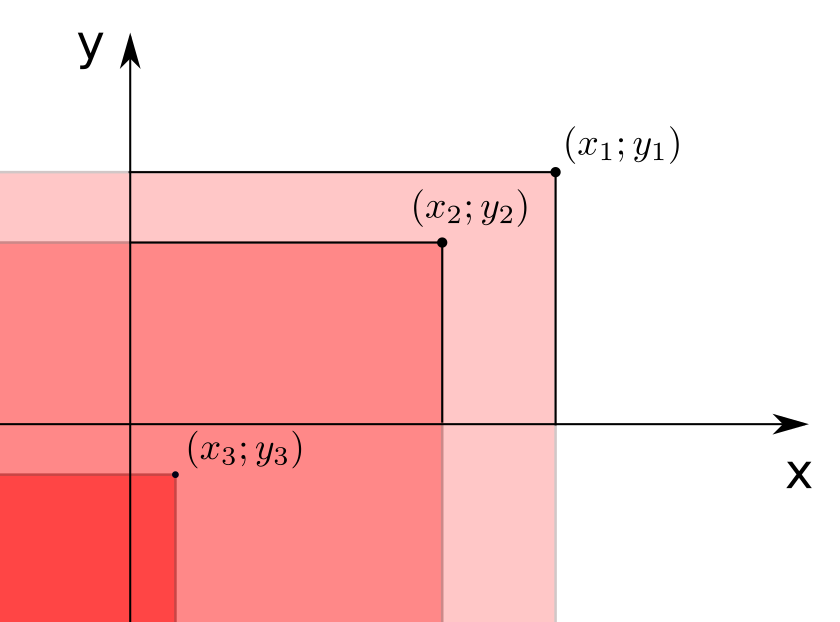
\includegraphics[scale=0.24]{images/10.png}
\end{gathered}
$$
\begin{proof}
$  \lim\limits_{n\to  \infty}{ F_{ \overline{\xi}} (x_n, y_n)} = 0 $, якщо $ x_n \to \infty$ або $y_n \to \infty$.
$$ \lim\limits_{n\to  \infty}{ F_{\overline{\xi}} (x_n, y_n) } =   \lim\limits_{n \to  \infty}{ \mathbb{P} \left\lbrace \xi_1 < x_n , \xi_2 < y_n \right\rbrace} = \mathbb{P} \left\lbrace  \bigcap\limits_{n\geq 1} (\xi_1 < x_n, \xi_2 < y_n) \right\rbrace = \mathbb{P} \left\lbrace \emptyset \right\rbrace = 0$$

\end{proof}
4b.
$$
\qquad\qquad
\begin{gathered}
\lim\limits_{\tiny \begin{gathered}
 x\to  +\infty\\ y\to  +\infty
\end{gathered}}{ F_ {\overline{\xi}} (x,y)} =  1
\end{gathered} \qquad \qquad \qquad
\begin{gathered}
 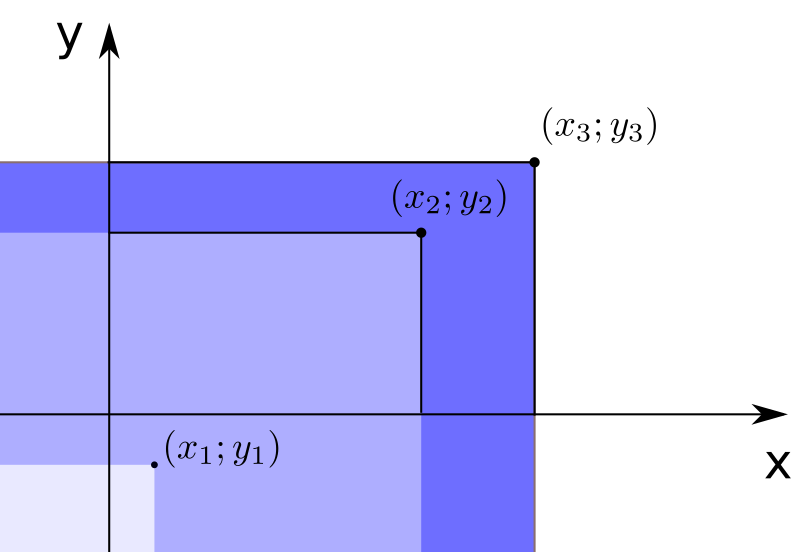
\includegraphics[scale=0.25]{images/11.png}
\end{gathered}
$$
\begin{proof}
$$
 \lim\limits_{n\to  \infty}{ F_{\overline{\xi}} (x_n, y_n) } =   \lim\limits_{n \to  \infty}{ \mathbb{P} \left\lbrace \xi_1 < x_n , \xi_2 < y_n \right\rbrace} = \mathbb{P} \left\lbrace  \bigcup\limits_{n\geq 1} (\xi_1 < x_n, \xi_2 < y_n) \right\rbrace = \mathbb{P} \left\lbrace \Omega \right\rbrace = 1
 $$
\end{proof}
4c.
$$
\lim\limits_{
\begin{gathered}
x\to  +\infty \\ y\in \mathbb{R}
\end{gathered}
}{ F_ {\overline{\xi}} (x,y)} =  \mathbb{P} \left\lbrace \xi_2 < y \right\rbrace = F_{\xi_2} (y)
$$

$$
\lim\limits_{
\begin{gathered}
y\to  +\infty \\ x\in \mathbb{R}
\end{gathered}
}{ F_ {\overline{\xi}} (x,y)} =  \mathbb{P} \left\lbrace \xi_1 < x \right\rbrace = F_{\xi_1} (x)
$$

\begin{defo}
$
\overline{\xi} = \begin{bmatrix}
 \xi_1 \\
 \xi_2
\end{bmatrix} \quad F_{\overline{\xi}} (x,y) - \textbf{сумісна функція розподілу.}
$\\
$\xi_1$ - випадкова величина. $ F_{\xi_1} $ -\textbf{маргінальна функція розподілу}  $ \xi_1$. \\ Щоб отримати маргінальну функцію розподілу, потрібно відправили ''зайві'' аргументи до $ + \infty$.\\
\end{defo}


5.  В одновимірному випадку:
$$
\qquad\quad
\begin{gathered}
\mathbb{P} \left\lbrace  \xi \in [a,b) \right\rbrace  = F_ \xi (b) - F_ \xi (a)
\end{gathered}\qquad \qquad
\begin{gathered}
 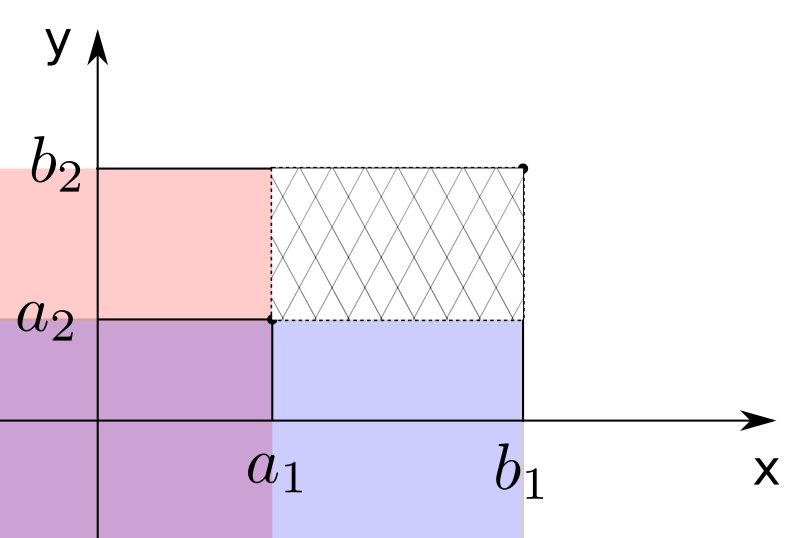
\includegraphics[scale=0.26]{images/6.png}\qquad
\end{gathered}$$
У багатовимірному випадку нас цікавить вірогідність $\mathbb{P} \left\lbrace \xi_1 \in [ a_1, b_1), \xi_2 \in [ a_2, b_2) \right\rbrace$ (користуємося правилом знаходження приросту функції 2-ох змінних):
$$\mathbb{P} \left\lbrace \xi_1 \in [ a_1, b_1), \xi_2 \in [ a_2, b_2) \right\rbrace = \mathbb{P} \left\lbrace \overline{\xi}  \in \text{ П}\right\rbrace =$$
$$
= F_{\overline{\xi}} (b_1, b_2) - F_{\overline{\xi}} (b_1, a_2)  - F_{\overline{\xi}} (b_1, a_2) + F_{\overline{\xi}} (a_1, a_2)
$$
\begin{example}
	$$
	\qquad\qquad
	F (x,y) = \left\lbrace
	\begin{gathered}
	 0, x+y \leq 0\\
	 1, x+y > 0
	\end{gathered} \right.
	\qquad \qquad
	\begin{gathered}
	 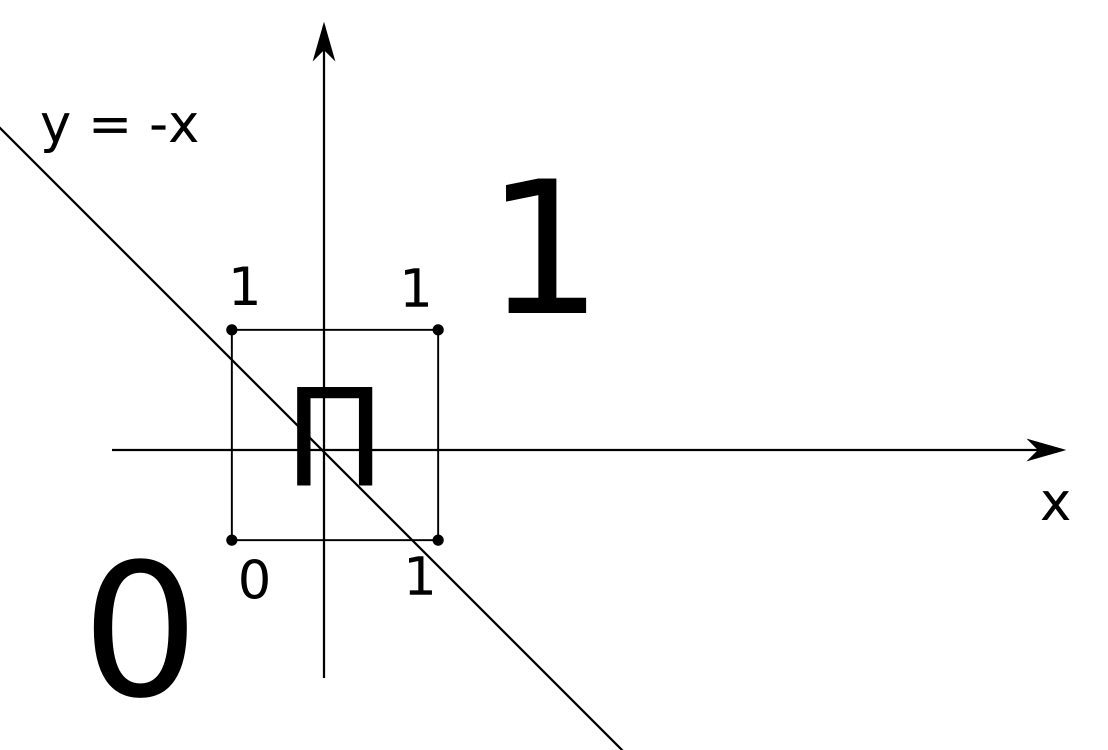
\includegraphics[scale=0.20]{images/12.png}\qquad
	 	\end{gathered}
	$$
	Задана функція не є функцією розподілу. Розглянемо прямокутник П.
\end{example}
\subsection{Дискретні та неперервні випадкові вектори.}
\subsubsection{Дискретні випадкові вектори.}
\begin{defo}
	$ \overline{\xi} = \begin{bmatrix}
	  \xi_1 \\
	...\\
	\xi_n\\
	\end{bmatrix}$ називають дискретним(неперервним), якщо усі його координати - дискретні(неперервні) випадкові величини.
\end{defo}
$
\overline{\xi} = \begin{bmatrix}
	\xi_1 \\
...\\
\xi_n\\
\end{bmatrix}
$ - дискретний вектор.
$p_{ij} = \mathbb{P} \left\lbrace \xi_1 = x_i , \xi_2= y_j \right\rbrace
\qquad $
$$
\begin{gathered}
 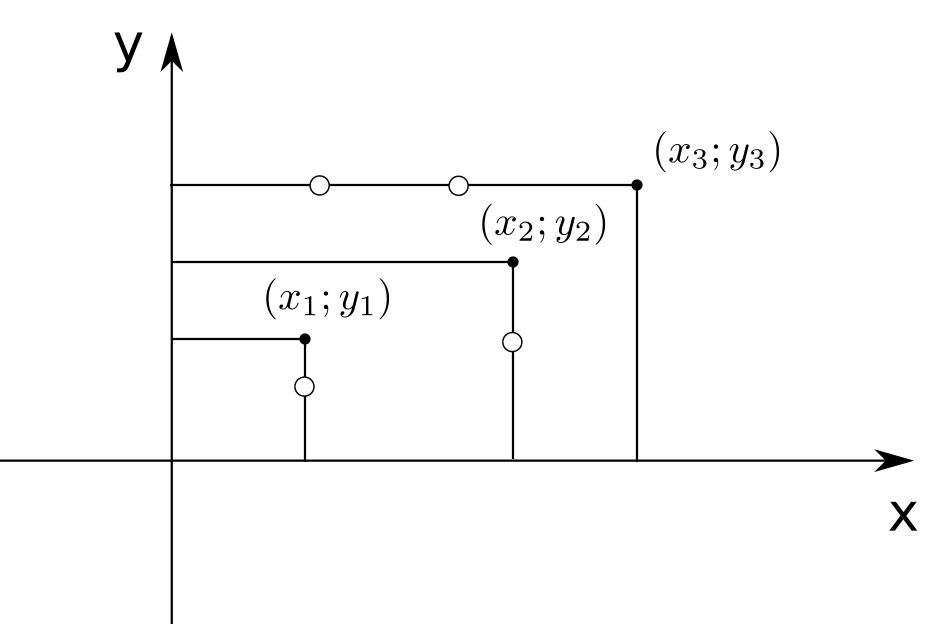
\includegraphics[scale=0.25]{images/13.png}\quad
	\end{gathered}
	\begin{gathered}
	 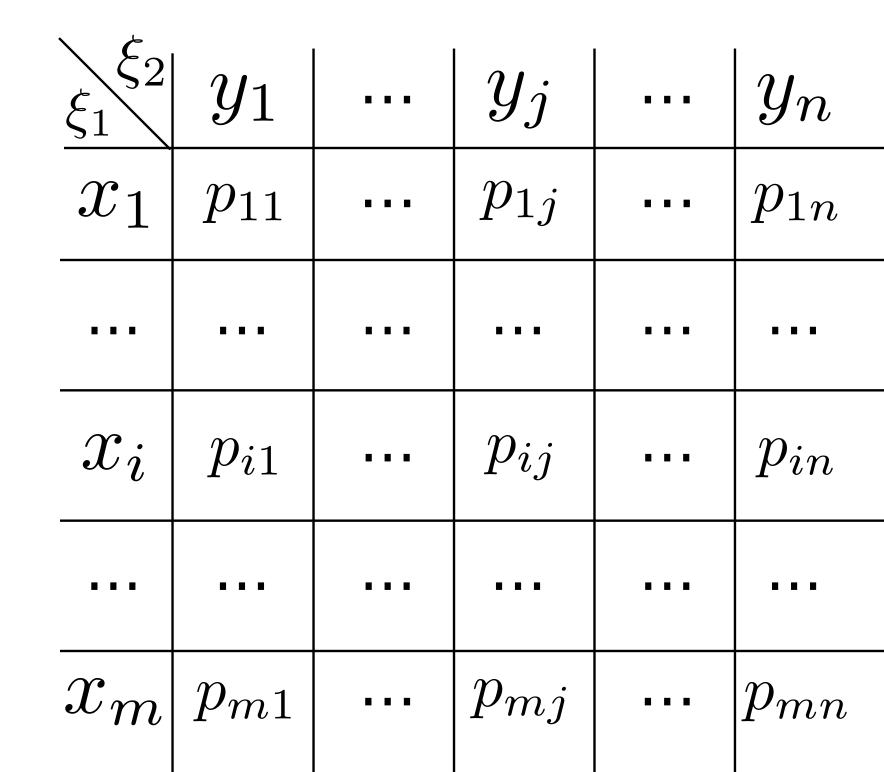
\includegraphics[scale=0.25]{images/14.png}\qquad
		\end{gathered}\qquad
$$
\subsubsection{Неперервні випадкові вектори.}
	$\xi$ - неперервна $ \Leftrightarrow$ $F_{\xi}$ - неп. функція $\Leftrightarrow$ $\mathbb{P} \left\lbrace \xi=x \right\rbrace  = 0 \quad \forall x \in \mathbb{R}$.
\begin{defo}
$ \overline{\xi}$ - неперервний вектор, якщо $ \mathbb{P} \left\lbrace  \xi = \overline{x} \right\rbrace = 0 \quad \forall  \overline{x}$
\end{defo}
\begin{defo}
	$ \overline{\xi}$ - абсолютно неперервний вектор, якщо $$ \exists f: F_{\xi} =  \int\limits_{-\infty}^{ x}{...  \int\limits_{-\infty}^{ x_n}{ f_{ \overline{\xi}}(x_1, ..., x_n)}dx_1...dx_n} = \mathbb{P} \left\lbrace \xi_1 < x_1 , ... , \xi_n < x_n\right\rbrace$$
	$$
	F_{\xi_1, \xi_2} (x,y) =  \int\limits_{- \infty}^{ x}{  \int\limits_{- \infty }^{ y}{ f_{\xi_1, \xi_2 }(s, t) dsdt}} \qquad \qquad
\begin{gathered}
  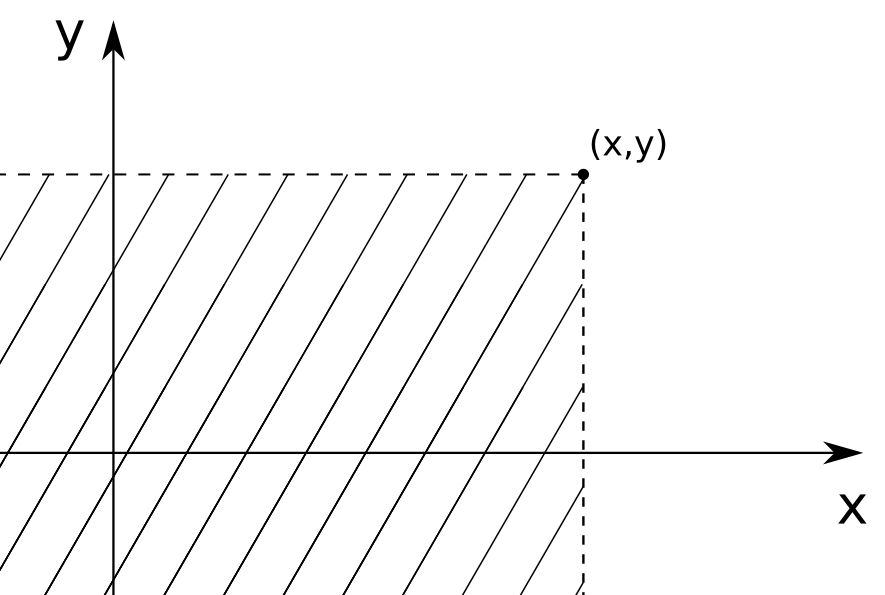
\includegraphics[scale=0.2]{images/15.png}
\end{gathered}
	$$

	\subsubsection{Властивості щільності розподілу:}
	1. $f_{\xi_1, \xi_2} (x,y) = \frac{ \partial ^2 F_{\xi_1, \xi_2}(x,y)}{ \partial x \partial y} $ - в точках, де похідна існує.\\
	2. $ \int\limits_{-\infty}^{ +\infty}{   \int\limits_{-\infty}^{ +\infty}{
	f_{\xi_1, \xi_2}(x,y) dxdy = 1
	}}$
	\begin{proof}
$$
 \lim\limits_{			\tiny
 \begin{gathered}
	    x\to  \infty\\
		 y\to \infty
	  \end{gathered}}{  \int\limits_{-\infty}^{ x}{   \int\limits_{-\infty}^{ y}{
		f_{\xi_1, \xi_2}(x,y) dxdy = 1} }} $$
		$$
		F_{\xi_1, \xi_2} (x,y) \begin{gathered}
		   \\
			\longrightarrow \\
			x,y\to \infty
		\end{gathered} 1
		$$
	\end{proof}
\end{defo}
3. $ \mathbb{P} \left\lbrace \overline{\xi} \in B \right\rbrace =  \iint\limits_{B}^{}{
f_{\overline{\xi}}dxdy}$, якщо $B$ - квадрована множина.
\begin{proof} Доведемо спочатку для прямокутників $ B = [a_1, b_1] \times [a_2, b_2]$.
  $$\mathbb{P} \left\lbrace \overline{\xi} \in B \right\rbrace = F(b_1, b_2) - F(b_1, a_2) - F(a_1, b_2) + F(a_2, b_2) =  \iint\limits_{B}^{}{ f_{ \overline{\xi}} dxdy}$$
\end{proof}
\subsection{Рівномірний розподіл на площині.}
$$
\overline{\xi} \sim U(A) \Leftrightarrow  f_{ \overline{\xi}} = \left\lbrace
\begin{gathered}
 c, (x,y) \in A\\
 0, (x,y)\notin A
\end{gathered} \right. \qquad \qquad
\begin{gathered}
 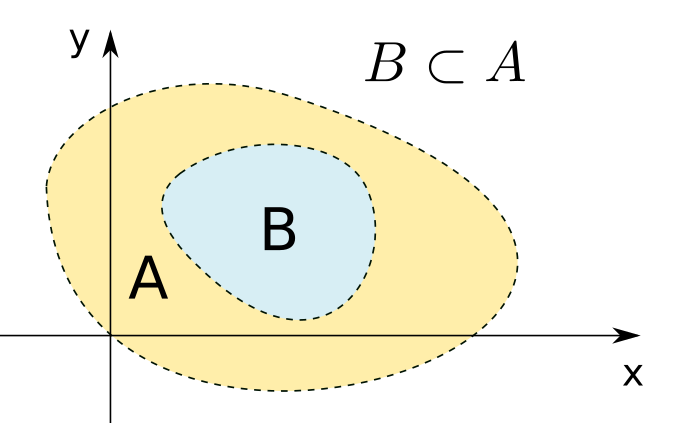
\includegraphics[scale=0.3]{images/16.png}
\end{gathered}
$$
$$
1 = \iint\limits_{\mathbb{R}^2	}^{}{
f_{\xi} (x,y )dxdy = c \cdot S(A) \Rightarrow c = \frac{1}{S(A)}
}$$
\begin{center}
\fbox{
 $
 f_{\overline{ \xi}} = \left\lbrace
 \begin{gathered}
	 \frac{1}{S(A)}, (x,y) \in A\\
	0, (x,y)\notin A
 \end{gathered} \right.
	$
}
\end{center}
$$
\mathbb{P} \left\lbrace \overline{\xi} \in B \right\rbrace = \iint\limits_{B}^{}{ f_{ \overline{ \xi}(x,y)}dxdy} = \iint\limits_{B}^{}{ \frac{1}{S(A)} } dxdy = \frac{S(B)}{S(A)}
$$
\subsection{Маргінальна щільність}
$$
\overline{\xi}  = \begin{bmatrix}
  \xi_1 \\ \xi_2
\end{bmatrix}
\qquad f_{ \overline{ \xi}} \text{ - щільність} \qquad f_{ \overline{ \xi}} (x) =  \int\limits_{- \infty}^{ +\infty}{ f_{ \overline{\xi}}(x,y)dy}
$$

\begin{proof}
$$ \int\limits_{C}^{}{f_{ \xi_1} dx}=
\mathbb{P} \left\lbrace \xi_1 \in C \right\rbrace = \mathbb{P} \left\lbrace ( \xi_1 , \xi_2 ) \in C \times \mathbb{R} \right\rbrace =  \int\limits_{C}^{}{   \int\limits_{-\infty}^{ +\infty}{ f_{ \overline{\xi}}(x,y) dxdy}}$$
\end{proof}

\begin{example}
$$	f_{ \overline{xi}} (x,y) = \left\lbrace  \begin{gathered}
3 , (x,y) \in D\\
0, (x,y) \notin D
	\end{gathered} \right. $$
	За умовою нормування:
	$$
	\begin{gathered}
		S(D) =  \int\limits_{0}^{1}{ ( \sqrt{x} - x^2 ) dx}= ( \frac{2}{3} x^{ \frac{3}{2} } - \frac{x^3}{3}  ) \Big|_0^1 = \frac{1}{3}\\
	f_{\xi} (x) =  \int\limits_{-\infty}^{ +\infty}{ f_{ \overline{\xi}} dy}
	\end{gathered}\qquad
	\begin{gathered}
	 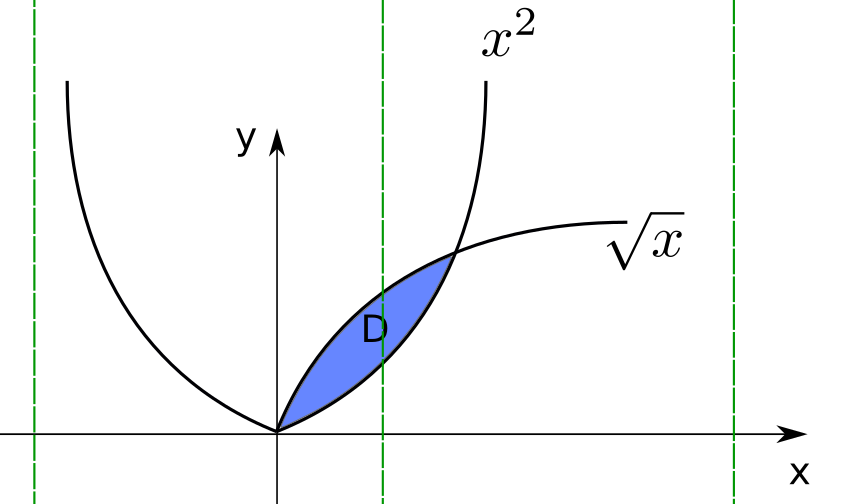
\includegraphics[scale=0.25]{images/17.png}
	\end{gathered}
	$$
	1. $ \begin{gathered}
	 x \in (-\infty; 0)\\
	 x \in (1; + \infty)
	\end{gathered} \quad f_{\xi_1} (x) =   \int\limits_{-\infty}^{ +\infty}{ 0dy} = 0$\\
	2. $x \in [0,1] \quad f_{\xi_1} (x) =   \int\limits_{x^2}^{ \sqrt{x}}{ 3dy} = 3 ( \sqrt{x} - x^2)$
	$$
	f_{\xi_1} (x) = \left\lbrace
\begin{gathered}
 0, x \in (-\infty, 0) \cup (1, +\infty ) \\
  3 ( \sqrt{x} - x^2), x \in [0,1]
\end{gathered}
	 \right.
	$$
	Перевірка: $  \int\limits_{-\infty}^{ +\infty}{ f_{\xi_1 } dx} = 3
	 \int\limits_{0}^{1}{ (\sqrt{x} - x^2)dx} = 1$ .\\
	 Аналогічно для $ f_{\xi_2} (y)$.
\end{example}

\subsection{Числові характеристики випадкових векторів.}
$$
\mathbb{E} \xi_1 =  \int\limits_{-\infty}^{ +\infty}{ x f_{\xi} (x) dx} =  \int\limits_{-\infty}^{ +\infty}{
\left( x
 \int\limits_{-\infty}^{ +\infty}{ f_{ \overline{ \xi}}  (x,y)dy}
 \right)dx =  \int\limits_{-\infty}^{ +\infty}{  \int\limits_{
 -\infty
 }^{ +\infty}{
 x f_{ \overline{ \xi}} (x,y) dxdy
 }}
}
$$
$$
\mathbb{E} \xi_2 =   \int\limits_{-\infty}^{ +\infty}{  \int\limits_{
-\infty
}^{ +\infty}{
y^2 f_{ \overline{ \xi}} (x,y) dxdy
}} =  \int\limits_{-\infty}^{ +\infty}{ dy \int\limits_{
-\infty
}^{ +\infty}{
y^2 f_{ \overline{ \xi}} (x,y) dx
}}  =  \int\limits_{-\infty}^{ +\infty}{ dx \int\limits_{
-\infty
}^{ +\infty}{
y^2 f_{ \overline{ \xi}} (x,y) dy
}}
$$
Таким чином, за подвійним інтегралом рахувати числові характеристики зручніше, адже ми можемо вибрати найпростіший вигляд.

\begin{example}
	Точка розподілена в одиничному крузі, для якого $f_ { \overline{\xi}} (x,y)$ пропорційеа відстані до границі круга. Знайти $ \mathbb{D} \xi_1, \mathbb{D} \xi_2$.
	$$
	f_{ \overline{ \xi}}(x,y) =
	\left\lbrace
	\begin{gathered}
	 (1 - \sqrt{x^2 + y^2})k, (x,y) \in \bigcirc \\
	  0 , (x,y) \notin \bigcirc
	\end{gathered} \right.\qquad
	\begin{gathered}
	 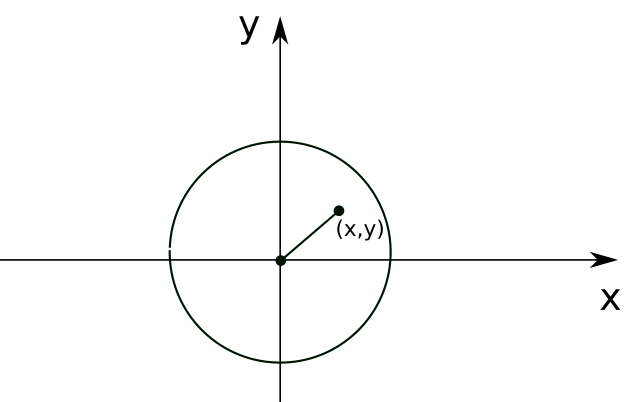
\includegraphics[scale=0.3]{images/18.png}
	\end{gathered}
	$$
	$$
	 1 = k \iint\limits_{\bigcirc}  ( 1 - \sqrt{x^2 + y^2})dxdy = k  \int\limits_{0}^{2\pi}{ d \varphi  \int\limits_{0}^{ 1}{ (1 - \rho)\rho d \rho}} =  \frac{\pi k}{3}  \Longrightarrow k = \frac{3}{\pi}
	$$
	$$
	\mathbb{D}\xi_1 = \mathbb{E} (\xi^2) - (\mathbb{E} \xi)^2 =  \iint\limits_{\bigcirc}^{ } x^2 \frac{3
	}{\pi} (1 - \sqrt{x^2 + y^2})dxdy
	$$
\end{example}

\subsection{Коваріація та її властивості.}
$$
\begin{gathered}
\overline{\xi} = \begin{bmatrix}
 \xi_1 \\
 \xi_2
\end{bmatrix} \qquad \mathbb{E}\xi_1, \mathbb{E}\xi_2. \mathbb{D}\xi_1, \mathbb{D}\xi_2
\end{gathered}
\qquad
\begin{gathered}
 
\includegraphics[scale=0.25]{images/19.png}\\
 \text{Маэстро, что с Вами?}
\end{gathered}
$$

\begin{defo}
	Коваріація (кореляційний момент) - $ cov( \xi_1, \xi_2)$.
	$$ cov(\xi_1, \xi_2 ) = \mathbb{E}(\xi_1 - \mathbb{E} \xi_2)(\xi_2 - \mathbb{E}\xi_2) = \mathbb{E}(\xi_1 \xi_2) - \mathbb{E} \xi_1 \xi_2$$
\end{defo}
\textbf{Коваріяція дискретного випадкового вектора.}
$$
cov( \xi_1, \xi_2) = \sum\limits_{i = 1}^{ m}{
 \sum\limits_{j = 1}^{ n}{ x_i \cdot y_j \cdot p_{ij}}
} - \left\lbrace  \sum\limits_{i = 1}^{ m}{
 \sum\limits_{j = 1}^{ n}{ x_i p_{ij}}
} \right\rbrace
\cdot
\left\lbrace \sum\limits_{i = 1}^{ m}{
 \sum\limits_{j = 1}^{ n}{ y_j p_{ij}}
} \right\rbrace
$$
\textbf{Коваріяція неперервного випадкового вектора.}
$$
cov( \xi_1 , \xi_2)=  \iint\limits_{\mathbb{R}^2	}^{ }{ xy  \cdot f_{ \overline{\xi}}  dxdy} - \iint\limits_{\mathbb{R}^2	}^{ }{ x  \cdot f_{ \overline{\xi}}  dxdy} \cdot \iint\limits_{\mathbb{R}^2	}^{ }{ y  \cdot f_{ \overline{\xi}}  dxdy}
$$
\begin{center}
\textbf{Властивості коваріації.}
\end{center}

1. $cov(\xi, \xi)  = \mathbb{D} \xi$.\\
2. Якщо $\xi_1, \xi_2 $ - незалежні , то $ cov( \xi_1 , \xi_2) = \mathbb{E}(\xi_1 - \mathbb{E}\xi_1) (\xi_2 - \mathbb{E}\xi_2) = 0$
\begin{defo}
	$\xi_1$ та $\xi_2$ наз. некорельованими,  якщо $ cov(\xi_1, \xi_2) =0$.
	\end{defo}

3. $ cov(\xi_1, \xi_2 ) = cov(\xi_2, \xi_1)$ (симетричність).\\
4. $cov(\xi, c) = 0$\\
5. $cov( \alpha \xi_1' + \beta \xi_1'', \xi_2) = \mathbb{E}( \alpha \xi_1' + \beta \xi_1 ''- \mathbb{E}(\alpha \xi_1' + \beta \xi_1 ''))
(\xi_2 - \mathbb{E}\xi_2) = \alpha cov(\xi_1', \xi_2) + \beta cov(\xi_1'', \xi_2)$\\
\textbf{Отримали:} Коваріація є білінійним симетричним функціоналом.\\
6. Якщо $\xi_1, \xi_2$ - незалежні, то  $\mathbb{D}(\xi_1 \pm \xi_2) = \mathbb{D}\xi_1 \pm \mathbb{D}\xi_2$.\\
Якщо існує залежність: $ \mathbb{D}( \xi_1 \pm \xi_2) = \mathbb{E}( (\xi_1 \pm \xi_2) - \mathbb{E}(\xi_1 \pm \xi_2))^2 = \mathbb{E}( (\xi_1 - \mathbb{E}\xi_1) \pm (\xi_2 - \mathbb{E}\xi_2)) = \mathbb{E}((\xi_1 - \mathbb{E} \xi_1)^2 + (\xi_2 - \mathbb{E} \xi_2 )^2 \pm 2 (\xi_1 - \mathbb{E} \xi_1)(\xi_2 - \mathbb{E}\xi_2)) =
\mathbb{D}\xi_1 + \mathbb{D}\xi_2  \pm 2cov(\xi_1, \xi_2)$
\\
7. $cov(\mathbb{I}_A, \mathbb{I}_B) = \mathbb{E} (\mathbb{I}_A \mathbb{I}_B) - \left( \mathbb{E} \mathbb{I}_A \right) (\mathbb{E} \mathbb{I}_B) = \mathbb{P} \left\lbrace A \cap B \right\rbrace - \mathbb{P} \left\lbrace A \right\rbrace \mathbb{P} \left\lbrace B  \right\rbrace$\\
8. Нерівність Коші-Буняковського.
$$
\left| cov(\xi_1, \xi_2) \right| \leq \sqrt{	\mathbb{D}\xi_1\cdot \mathbb{D}\xi_2}
$$

\subsection{Коваріаційна матриця вектора та її властивості}

$\xi: $ дисперсія $\mathbb{D} \xi = \mathbb{R}\mathbb{E} (\xi - \mathbb{E}\xi)^2$\\
$ \overline{\xi}: $ коваріаційна матриця $C_{ \overline{\xi}} = \mathbb{E}( \overline{\xi} - \mathbb{E}\overline{\xi})(\overline{\xi} - \mathbb{E} \overline{\xi})^T$
$$
C_{ \overline{\xi}} = \begin{bmatrix}
 \mathbb{D} \xi_1 & cov(\xi_1, \xi_2) & \cdots & cov(\xi_1, \xi_n) \\
 cov(\xi_2, \xi_1) & \mathbb{D}\xi_2 & \cdots & cov(\xi_2, \xi_n)\\
 \vdots & \vdots & \ddots & \vdots\\
 cov(\xi_n, \xi_1)& cov(\xi_n, \xi_1) & \cdots & \mathbb{D}\xi_n
\end{bmatrix}
$$
1. $C_{\overline{\xi}}$ - симетрична матриця.\\
2. $A$ - квадратна матриця $n \times n$, симетрична.\\$A$ - невід'ємно визначена $\Leftrightarrow (A \overline{x}, \overline{x}) \geq \forall  \overline{x} \in \mathbb{R}^n$
$C_{\overline{\xi}}$ - невід'ємно визначена. $ (C_{\overline{\xi}}, \overline{\xi}) = (\mathbb{E}(\overline{\xi} - \mathbb{E}\overline{\xi})(\mathbb{E}(\overline{\xi} - \mathbb{E}\overline{\xi})^T \overline{x}, \overline{x} ) = \mathbb{E} \left| \left| (\overline{\xi} - \mathbb{E} \overline{\xi})^T \overline{x}\right| \right|^2 \geq 0 $.\\
Застосування невід'ємної визначеності.
$$
\overline{\xi} = \begin{bmatrix}
 \xi_1\\
 \xi_2
\end{bmatrix} \qquad \qquad C_{ \overline{\xi}} = \begin{bmatrix}
 \mathbb{D}\xi_1 & cov(\xi_1, \xi_2) \\
 cov(\xi_1, \xi_2) & \mathbb{D} \xi_2
\end{bmatrix} - \text{ невід'ємно визначена}
$$
Застосуємо критерій Сільвестра:
$$
\mathbb{D}\xi_1 \cdot \mathbb{D}\xi_2 - cov^2(\xi_1, \xi(2)) \geq 0 \Longrightarrow  \left| cov(\xi_1, \xi_2) \right| \leq \sqrt{ \mathbb{D} \xi_1 \cdot \mathbb{D}\xi_2}
$$


\textbf{Що означає виродженість коваріаційної матриці?} $ \Leftrightarrow \det C_{ \overline{\xi}} = 0$:
$$
\det C_{ \overline{\xi}} = 0 \Leftrightarrow \exists \overline{x} \in \mathbb{R}^n: \left( C_{\overline{\xi}}, \overline{\xi} \right) = 0
\Leftrightarrow C_{ \overline{\xi}} - \text{не додатня, невід'ємно визначена}
$$
\begin{proof}
$$
\det C_{ \overline{\xi}} = 0 \Rightarrow Ker C_{ \overline{\xi}} \neq \left\lbrace \vec{0} \right\rbrace \Rightarrow \exists \overline{x} \neq 0: C_{ \overline{\xi}} \overline{x} = 0\Rightarrow \left( C_{\overline{\xi}} \overline{x}, \overline{x} \right) = 0
$$
$$
\exists \overline{x} \neq 0: \left( C_{\overline{\xi}} \overline{x}, \overline{x} \right) = 0 \Rightarrow \exists \overline{y} \neq 0: \lambda_1 y_1^2 + ... + \lambda_n y_n^2
$$
$$
\left( C_{\overline{\xi}} \overline{x}, \overline{x} \right) = 0 = \left( \Omega \overline{y}, \overline{y} \right) = \lambda_1 y_1^2 + ... + \lambda_n y_n^2\Leftrightarrow \exists \lambda_i = 0 \Rightarrow \det C_{ \overline{\xi}} = 0
$$
\end{proof}
\begin{boxteo}
	$C_{\overline{\xi}}$ є виродженою т.т.т.к між $ \xi_1, ... , \xi_n$ є афінна залежність. Тобто:
	$$\lambda_1 \xi_1 + \lambda_2 \xi_2 +...+ \lambda_n \xi_n = c$$
\end{boxteo}
\begin{proof}
 $$
\exists \overline{x} \neq 0: \left( C_{\overline{\xi}} \overline{x}, \overline{x} \right) = 0 \Leftrightarrow \exists \overline{ \xi} \neq \vec{0} \in \mathbb{R}^n: \left( \mathbb{E}( \overline{\xi} - \mathbb{E}\overline{\xi})(\overline{\xi} - \mathbb{E} \overline{\xi})^T \cdot \overline{x}, \overline{x} \right) = 0 \Leftrightarrow
 $$
 $$
\Leftrightarrow  \left( \mathbb{E}( \overline{\xi} - \mathbb{E}\overline{\xi}) \cdot \overline{x},(\overline{\xi} - \mathbb{E} \overline{\xi})\cdot \overline{x} \right) = 0 \Leftrightarrow
 $$
 $$
 \Leftrightarrow \mathbb{E} \left| \left|  \left( \overline{\xi} - \mathbb{E}\overline{\xi} \right)^T \overline{x}  \right|  \right|^2 = 0 \Leftrightarrow \left| \left|  \left( \overline{\xi} - \mathbb{E}\overline{\xi} \right)^T \overline{x}  \right|  \right|^2 = 0 \quad \text{м.н.}
\Leftrightarrow $$
$$
\Leftrightarrow\left( \overline{\xi} - \mathbb{E}\overline{\xi} \right)^T \overline{x} = 0 \Leftrightarrow \left( \xi_1 - \mathbb{E} \xi_1 \right) x_1 + ... + (\xi_n - \mathbb{E}\xi_n) x_n = 0 \Leftrightarrow
$$
$ \exists x_1, ..., x_n$ не всі з яких дорівнюють нулю:
$$
\Leftrightarrow
x_1 \xi_1 + x_2 \xi_2 + ... + x_n \xi_n  = x_1 \mathbb{E}\xi_1 + ... + x_n \mathbb{E}\xi_n = c
\Leftrightarrow
$$
Візьмемо $ x_i = \lambda_i$: $ \lambda_1 \xi_1 + ... + \lambda_n \xi_n = c \Leftrightarrow$ афінна залежність.
\end{proof}

Розглянемо $
cov( \xi, \eta) = \mathbb{E}(\xi - \mathbb{E}\xi) (\eta - \mathbb{E}\eta)
$.\\
Застосуємо нерівність Коші-Буняковського:
$ \left| cov(\xi, \eta) \right| \leq \sqrt{ \mathbb{D}\xi \cdot\mathbb{D}\eta} $
\begin{center}
\fbox{
	$r_{\xi, \eta} =\displaystyle\frac{cov(\xi, \eta)}{\sqrt{\mathbb{D}\xi\cdot \mathbb{D}\eta}} $ - коефіцієнт кореляції між $\xi$ та $\eta$.
}\\
\end{center}
$$-1 \leq r_{\xi, \eta} \leq 1 $$

Коефіцієнт показує ''силу'' лінійної залежності між $\xi$ та $\eta$.
$$
r_{\xi, \eta } = 0 \Leftrightarrow cov(\xi, \eta) \Leftrightarrow \xi \text{ та } \eta  \text{- некорельовані.}
$$
$$
r_{\xi, \eta}= \pm 1  \Leftrightarrow \det \begin{bmatrix}
 \mathbb{D} \xi & cov(\xi, \eta)\\
 cov(\xi, \eta) & \mathbb{D} \eta
\end{bmatrix} = 0 \Leftrightarrow \det C_{\xi, \eta} = 0\Leftrightarrow
$$
$$
\Leftrightarrow \mathbb{D}\xi \cdot \mathbb{D}\eta - cov(\xi, \eta) = 0 \Leftrightarrow \left| r_{\xi, \eta}  \right| = 1
$$
\begin{boxteo}
	$r_{\xi, \eta}= \pm 1$ т.т.т.к. $\eta = k \xi + b$, де $k, b \in R$\\
	При цьому $\begin{gathered}
	 r_{\xi, \eta} +1 \Rightarrow k>0\\
	 r_{\xi, \eta} -1 \Rightarrow k<0
	\end{gathered}$
\end{boxteo}
\begin{proof}
 $$r_{\xi, \eta} = \frac{cov(\xi, k \xi +b)}{\mathbb{D}\xi\cdot \mathbb{D}(k \xi +b)} = \frac{k \mathbb{D}\xi}{ \sqrt{k^2 \cdot \mathbb{D}^2 \xi} }  = \frac{k}{ \left| k \right| } = \left\lbrace \begin{gathered}
  1, k>0\\
	-1, k<0\\
 \end{gathered} \right. $$
\end{proof}
\subsection{Незалежність випадкових величин}
\begin{defo}
	Випадкові величини $\xi, \eta$ називають незалежними, якщо події \\$ \left\lbrace \xi\in [a,b] \right\rbrace, \left\lbrace \eta\in [a,b] \right\rbrace $ є незалежними $ \forall a \leq  b , c\leq d$\\
	Зокрема, якщо $\xi, \eta$ - дискретні:
	$$
	\begin{gathered}
	 \xi \in \left\lbrace x_1, ..., x_n \right\rbrace\\
	 \eta \in \left\lbrace y_1, ..., y_n  \right\rbrace
	\end{gathered} \qquad \left\lbrace \xi = x_i \right\rbrace \independent \left\lbrace \eta = y_j \right\rbrace \quad \begin{gathered}
	 \forall i = \overline{1, m}\\
	 \forall j = \overline{1, n}
	\end{gathered}
	$$

\end{defo}

\pagebreak

\begin{boxteo}
	$\xi, \eta$ - незалежні $\Leftrightarrow F_{\xi, \eta} = F_{\xi}(x) \cdot F_{\eta}(y)$
\end{boxteo}
\begin{proof}
Нехай $\xi, \eta$ - незалежні $\Leftrightarrow \forall a\leq b, c\leq d: \mathbb{P} \left\lbrace  \xi \in [a,b], \eta \in [c,d] \right\rbrace = \mathbb{P} \left\lbrace \xi\in[a,b] \right\rbrace \cdot \mathbb{P} \left\lbrace \eta\in[c,d] \right\rbrace \Rightarrow \mathbb{P} \left\lbrace  \xi\in [a,b), \eta \in [c,d) \right\rbrace = \mathbb{P} \left\lbrace \xi \in [a,b) \right\rbrace \cdot \mathbb{P} \left\lbrace \eta \in [c,d) \right\rbrace  $\\
$
\mathbb{P} \left\lbrace \xi<b, \eta <d  \right\rbrace = \mathbb{P} \left\lbrace \xi < b \right\rbrace \cdot \mathbb{P} \left\lbrace \eta <d \right\rbrace \Leftrightarrow F_{\xi, \eta} (b,d) = F_{\xi}(b) \cdot F(\eta)(d)
$\\
Нехай навпаки: $ F_{\xi, \eta } (x,y)  = F_{\xi}(x) - F_{\eta}(y)\quad \forall x,y \in \mathbb{R}$
$$
\mathbb{P} \left\lbrace  \xi\in [a,b), \eta \in [c,d)\right\rbrace = F_{\xi, \eta} (d,b) - F_{\xi,\eta}(b,c) - F_{\xi, \eta }(a,d) + F_{\xi, \eta}(a,c) =
$$
$$
= F_{\xi}(b) F_{\eta} (d) - F_{\xi}(b) F_{\eta}(c) - F_{\xi}(a) F_{\eta}(d) + F_{\xi}(a) F_{\eta}(c)  =$$


$$= \left( F_{\xi}(b) - F_{\xi}(a) \right) \left( F_{\eta}(d) - F_\eta (c) \right) = \mathbb{P} \left\lbrace \xi\in [a,b) \right\rbrace \cdot \mathbb{P} \left\lbrace \eta \in [c,b) \right\rbrace
$$

\end{proof}
\begin{boxteo}Для абсолюно неперервного векторa $\begin{bmatrix}
	 \xi& \eta
	\end{bmatrix}^T$\\
$$\xi \independent \eta \Leftrightarrow f_{\xi, \eta} (x,y)= f_{\xi}(x) f_{\eta}(y) \quad \forall x,y \in \mathbb{R}$$
\end{boxteo}

\begin{proof}
$$
\begin{gathered}
1. \quad  F_{\xi, \eta} (x,y) = F_{\xi}(x) \cdot F_{\eta}(y) \Longrightarrow f_{\xi, \eta} (x,y) = f_{\xi}(x) \cdot f_{\eta}(y)\\
	2. \quad f_{\xi, \eta} (x,y) = f_{\xi}(x) \cdot f_{\eta}(y)\Longrightarrow F_{\xi, \eta} (x,y) = F_{\xi}(x) \cdot F_{\eta}(y)
\end{gathered}\quad \forall x,y \in \mathbb{R}
$$
\end{proof}


\newpage
% N-integrals by R^n - \underset{R^n}{ \int \cdots \int}

\section{Функції від випадкових величин (векторів)}
Для дискретної випадкової величини $\xi$: $\eta = \phi (\xi) \Rightarrow \eta$ - ДВВ. \\
Припустимо, що $\varphi$ - неперервно диференційована. $\xi$ - асолютно неперервна зі щільністю $f_{\xi}(x)$. Розглядаємо $ \eta = \varphi(\xi) $:

\begin{boxteo}
    Нехай $\varphi$ - взаємно-однозначна (бієкція на області значень), та її обернена $\psi$ є неперервно диференційована. (Дифеоморфізм). Тоді:
    $$
    f_{\eta} (y) = \begin{cases}
    \left| \psi '(y) \right| \cdot  f_{\xi }(\psi (y)), & y \in E_{\varphi}\\
        0 & y \notin E_{\varphi}
    \end{cases} = f_{\xi} (\psi (y)) \cdot \left| \psi'(y) \right| \cdot \mathbb{I}_{E_{\varphi}}(y)
    $$
\end{boxteo}

\begin{proof}
Розглядаемо множину B.
$$  \int\limits_{B }^{ }{ f_{\eta} (y)dy} = \mathbb{P} \left\lbrace \eta \in B \right\rbrace =
\mathbb{P} \left\lbrace \varphi(\xi) \in B \right\rbrace = \mathbb{P} \left\lbrace \xi \in \phi^{-1} (B) \right\rbrace =  \int\limits_{\phi^{-1} (B)}^{}{f_{\xi}(x)dx} =
$$
$$
= \left| \begin{gathered}
  \varphi(x) = y \\
  x = \psi(y)
  % \\J = \psi'(y) = J_{\psi}
\end{gathered} \right|  =  \int\limits_{B \cap E_{\varphi}}^{ }{ f_{\xi} (\psi (y)) \cdot \left| J_{\psi} (y)  \right| dy} =  \int\limits_{B}^{ }{f_{\xi} (\psi (y)) \cdot \left| \psi'(y) \right| \cdot \mathbb{I}_{E_{\varphi}}(y)dy}
$$
\end{proof}
\begin{boxteo}
Нехай $\phi$ не є ін'єкцією, але ''розпадається'' на декілька таких.
$$
\begin{gathered}
 \varphi_1 (x) = x^2, x\in (- \i, 0)\\
 \varphi_2(x) = x^2, x \in [0, +\i]\\
 E_{\varphi_1} = (0, + \i) \quad E_{\varphi_2} = (0, + \i)\\
 \psi (x) = y   \quad x^2 = y  \quad x = \pm \sqrt{y} \\
 \psi_1(y) = - \sqrt{y} \quad \psi_2(y) = \sqrt{y}
\end{gathered} \qquad \qquad
\begin{gathered}
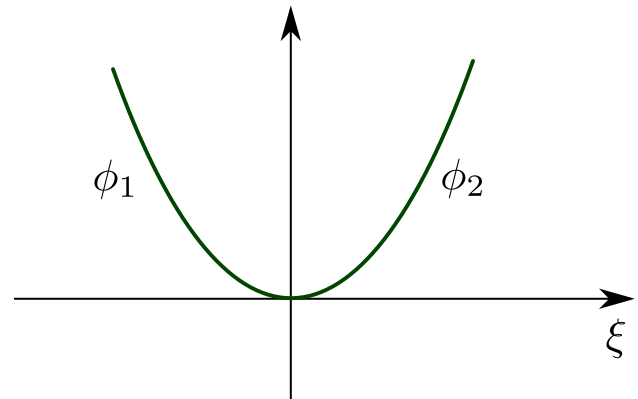
\includegraphics[scale=0.25]{assets/lectures_part_3-7a9fde69.png}
\end{gathered}
$$
\textbf{Тоді: } \fbox{$ f_{\eta} (y) =  \sum\limits_{i = 1}^{ n}{ f_{\xi} (\psi_i (y)) \cdot \left| \psi_i'(y) \right| \cdot \mathbb{I}_{E_{\varphi_i}}(y)}$}.
\end{boxteo}
\begin{proof}
  Розглядаемо множину B.
  $$  \int\limits_{B }^{ }{ f_{\eta} (y)dy} \!=\! \mathbb{P} \left\lbrace \eta \in B \right\rbrace \!=\!
 \mathbb{P} \left\lbrace \xi \in \phi_1^{-1} (B) \cup \cdots \cup \xi \in \phi_n^{-1} (B) \right\rbrace  \!=\!\! \sum\limits_{i = 1}^{n}{ \mathbb{P} \left\lbrace \xi \in \phi_i^{-1} (B) \right\rbrace  }
  $$
  \end{proof}

 \subsection{Функції від випадкових векторів.}
 Розглядаємо $ \overline{\xi} = \begin{bmatrix}
  \xi_1 \\
  \xi_2
 \end{bmatrix} \quad \eta = \varphi(\xi_1, \xi_2)$.\\
 1. Для дискретного випадку обчислення тривіальні.\\
 2. $ \overline{\xi} $ - абсолютно неперервний випадковий вектор.
 $$ f_{\overline{\xi}} (\overline{x}) \Rightarrow \eta = \varphi( \overline{\xi}) \quad f_{\eta} (y)=? \quad \varphi: \mathbb{R}^n \to \mathbb{R}$$
\begin{boxteo}
    $ \varphi: \mathbb{R}^n \to \mathbb{R}^n. \varphi$ - взаємно-однозначна $ \Rightarrow \psi = \varphi^{-1}$.\\
    $\varphi, \psi $ - дифеоморфізми $ \Rightarrow  \exists J_{\psi} ( \overline{y}) $ - якобіан. Тоді:
    $$
    f_{\overline{\eta}}  (\overline{y}) = f_{\overline{\xi}} (\psi(\overline{y})) \cdot \left| J_{\psi }(\overline{y}) \right| \cdot   \mathbb{I}_{E_{\varphi}} (\overline{y})
    $$
\end{boxteo}
\begin{boxteo}
    $\varphi$ розпадаэться на суму ін'єктивних функцій  $\varphi_1, ..., \varphi_k$.\\
    $ \varphi^{-1}_i = \psi_i. \quad E_i$ - область значень $ \varphi_i. \quad J_{\psi_i}$ - якобіан $ \psi_i$. Тоді:
    $$
    f_{\eta} (\overline{y}) =  \sum\limits_{i = 1}^{ k}{ f_{\overline{\xi}} ( \psi_i( \overline{y})) \cdot \left| J_{\varphi_i } (\overline{y}) \right|  \cdot \mathbb{I}_{E_{\varphi_i}} (\overline{y})}
    $$
\end{boxteo}
Часто будемо використовувати: \fbox{$f_{\xi_1 + \xi_2} (y) =  \int\limits_{-\infty}^{ +\infty}{ f_{\overline{\xi} } (x, y-x) dx}$}.\\
Якщо $ \xi_1 \independent \xi_2: $ \fbox{$ f_{\xi_1 + \xi_2} (y) =  \int\limits_{-\infty}^{ +\infty}{ f_{\xi_1} (x) \cdot f_{\xi_2} (y-x) dx}$}.\\ Також: $f_{\xi_1 + \xi_2} (y) = (f_{\xi_1}(x) \circledast f_{\xi2} (y))$ - згортка.
\subsection{Загальний алгоритм знаходження PDF}
Розглядаємо $ \eta = \varphi( \overline{\xi}) \quad f_{\eta} (z) = ?$.
$$
F_{\eta} = \mathbb{P} \left\lbrace  \eta < z \right\rbrace = \mathbb{P} \left\lbrace \varphi(\xi_1, \xi_2) < z \right\rbrace = \left| \left\lbrace (x,y) \in \mathbb{R} \Big| \varphi(x,y) < z \right\rbrace = D_z \right|  =
$$
$$
 =  \iint\limits_{D_z}^{}{f_{\overline{\xi} }(x,y ) dxdy} \Longrightarrow f_\eta (z)  = F_\eta' (z)
$$
Знайдемо щільності розподілу суми, добутку та частки випадкових величин.
$$\xi_1, \xi_2, f_{\overline{\xi} }(x,y) \Longrightarrow f_{\xi_1 + \xi_2} (z), f_{\xi_1 \cdot \xi_2} (x,y), f_{\xi_1/ \xi_2} (x,y) - ?$$
\textbf{Сума:} $ F_{\xi_1 + \xi_2} (z) = \mathbb{P} \left\lbrace \xi_1 + \xi_2 < z \right\rbrace = \mathbb{P} \left\lbrace \overline{\xi} \in D_z \right\rbrace =
  \iint\limits_{D_z}^{ }{ f_{\overline{\xi}} ( x,y) dxdy} =
$
$$
\begin{gathered}
=  \int\limits_{-\infty}^{ +\infty}{ dx  \int\limits_{-\infty}^{ z-x}{f_{\overline{\xi}}(x,y)dy}}\\
 f_{\xi_1 + \xi_2} (z) = \int\limits_{-\infty}^{ +\infty}{ f_{\overline{\xi}} (x, z-x) dx}
\end{gathered}\qquad \quad
\begin{gathered}
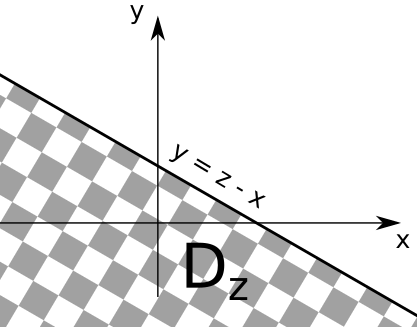
\includegraphics[scale=0.45]{assets/lectures_part_3-43a27a3a.png}
\end{gathered}
$$
$$
f_{\xi_1 + \xi_2} (z) =  \int\limits_{-\infty}^{ +\infty}{ f_{\overline{\xi}}(x, z-x)dx = \left| \xi_1 \independent \xi_2 \right| =  \int\limits_{-\infty}^{ +\infty}{ f_{\xi_1} (x) \cdot f_{\xi_2} (z-x) dx }}
$$
\textbf{Добуток: } Шукаємо $ f_{\xi_1 \cdot \xi_2 } \quad F_{\xi_1 \cdot \xi_2}= \mathbb{P} \left\lbrace \xi_1 \cdot \xi_2 < z \right\rbrace$.\\
$$
\begin{gathered}
x * y < z \Leftrightarrow \left[ \begin{gathered}
\begin{cases}
    y < \frac{z}{x}\\
    x> 0
\end{cases}\\
\begin{cases}
    y > \frac{z}{x}\\
    x < 0
\end{cases}
\end{gathered}
 \right.
\end{gathered}
 \qquad  \qquad  \quad
 \begin{gathered}
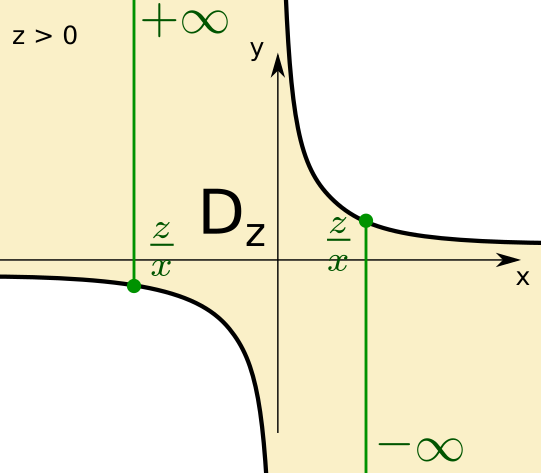
\includegraphics[scale=0.37]{assets/lectures_part_3-5c275c57.png}
 \end{gathered}
$$
$$
F_{\xi_1 \cdot \xi_2} (z) =  \iint\limits_{D_z}^{ }{ f_{\overline{\xi}} (x,y) dxdy} =  \int\limits_{-\infty}^{0}{dx  \int\limits_{ \frac{z}{x}  }^{ +\infty}{ f_{\overline{\xi}} (x,y )dy}} +  \int\limits_{0}^{ +\infty}{ dx  \int\limits_{-\infty}^{ \frac{z}{x} }{f_{\overline{\xi}} (x,y )dy}}
$$
$$
f_{\xi_1 \cdot \xi_2} (z) = -  \int\limits_{-\infty}^{ 0}{ f_{\overline{\xi}}(x, \frac{z}{x})\cdot \frac{1}{x} dx  } + \int\limits_{0}^{ + \infty}{ f_{\overline{\xi}}(x, \frac{z}{x})\cdot \frac{1}{x} dx  }
$$

\textbf{Відношення.} Розглядаємо: $\overline{\xi} = \begin{bmatrix}
 \xi_1 \\
 \xi_2
\end{bmatrix} \quad f_{\overline{\xi}} (x,y) \quad \eta = \frac{\xi_2}{\xi1} $. За алгоритмом:
$$
F_{\eta} (z) = \mathbb{P} \left\lbrace \frac{\xi_2}{\xi_1} <z  \right\rbrace = \mathbb{P} \left\lbrace \overline{\xi} \in D_z \right\rbrace =  \iint\limits_{D_z}^{}{ f_{\overline{\xi}}(x,y)dxdy}
$$
де, $ D_z = \left\lbrace (x,y) \in \mathbb{R}^2| \frac{y}{x} < z  \right\rbrace $
Якщо $z > 0 :$
$$
\begin{gathered}
 \frac{y}{x} < z \Leftrightarrow
\left[
\begin{gathered}
\begin{cases}
    y < xz \\
    x > 0
\end{cases}
\\
\begin{cases}
    y > xz \\
    x < 0
\end{cases}
\end{gathered}
 \right.
 \qquad
\end{gathered}  \qquad  \qquad  \qquad
  \begin{gathered} 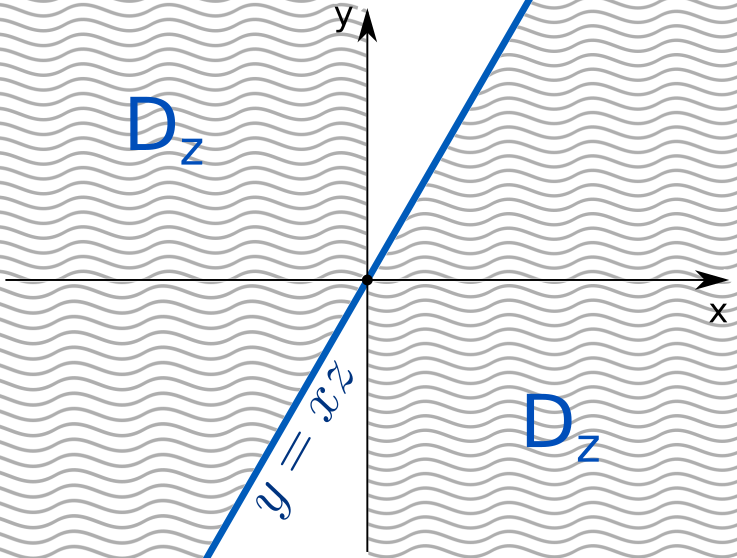
\includegraphics[scale=0.27]{assets/lectures_part_3-f7d7887c.png} \end{gathered}
$$
Повертаємося до інтегралу, що записано вище:
$$
F_{\eta} (z) =  \int\limits_{-\infty}^{0}{ dx   \int\limits_{zx}^{ +\infty}{ f_{\overline{\xi}}}(x,y) dy} +  \int\limits_{0}^{ +\infty}{ dx
 \int\limits_{-\infty}^{zx}{ f_{\overline{\xi}}(x,y) dy}
}
$$
$$
f_{\eta}(z) = F_{\eta}'(z) =  \int\limits_{-\infty}^{ 0}{ f_{\overline{\xi}}(x,zx)x dx} +  \int\limits_{0}^{ +\infty}{f_{\overline{\xi}}(x, zx) x dx}
$$
\begin{example}
    $\xi_1, \xi_2 \sim N(0,1) \quad \xi_1 \independent \xi_2 \quad \eta = \frac{\xi_2}{\xi_1} $
\\ Величини $\xi_1, \xi_2$ розподілені нормально: $
f_{\xi_1} (x) = \frac{1}{\sqrt{2 \pi}} e^{ - \frac{x^2}{2} }  = f_{\xi_2 } (x).
$
$$
f_{\eta} (z) = -  \int\limits_{-\infty}^{ 0}{\frac{1}{\sqrt{2 \pi}} e^{ - \frac{x^2}{2} } \cdot \frac{1}{\sqrt{2 \pi}} e^{ - \frac{z^2x^2}{2} } } x dx + \int\limits_{0}^{ +\infty}{\frac{1}{\sqrt{2 \pi}} e^{ - \frac{x^2}{2} } \cdot \frac{1}{\sqrt{2 \pi}} e^{ - \frac{z^2x^2}{2} } } x dx  =
$$
$$
= - \frac{1}{2\pi}  \int\limits_{-\infty}^{0}{ e^{ -\frac{x^2}{2}(1+z^2) }} \underbrace{xdx}_{= d \left( \frac{x^2}{2}  \right)}  + \frac{1}{2\pi}  \int\limits_{0}^{+ \infty}{ e^{ -\frac{x^2}{2}(1+z^2) }} \underbrace{xdx}_{= d \left( \frac{x^2}{2}  \right)} =
$$
$$
= - \frac{1 }{2 \pi ( 1 + z^2)}  \int\limits_{-\infty}^{0}{ e^{- \frac{x^2}{2}(1+z^2) } d \left( \frac{x^2}{2}(1+z^2) \right) }  + \frac{1 }{2 \pi ( 1 + z^2)}  \int\limits_{0}^{+ \infty}{ e^{- \frac{x^2}{2}(1+z^2) } d \left( \frac{x^2}{2}(1+z^2) \right) } =
$$
$$
= \frac{1 }{2 \pi ( 1 + z^2)}   e^{- \frac{x^2}{2}(s+z^2) } \Bigg|_{x = -\infty}^{0}  - \frac{1 }{2 \pi ( 1 + z^2)}   e^{- \frac{x^2}{2}(1+z^2) } \Bigg|_{x = 0}^{+\infty} =
$$
$$
 =\frac{1}{2\pi (1+ z^2)} +  \frac{1}{2\pi (1+ z^2)} = \frac{1}{\pi (1+ z^2)} , z \in \mathbb{R}
$$
Отримали, що: $ \dfrac{N(0,1)}{N(0,1)} \sim \textbf{Cauchy Distribution} $
\end{example}

\subsection{Щільності розподілу максимума, мінімума, порядкових статистик.}
\subsubsection{Максимум.}
Розглянемо максимум з деяких незалежних випадкових величин: $ \xi_1 , \xi_2, ... , \xi_n$.
$$M = \max \left\lbrace \xi_1, ..., \xi_n \right\rbrace $$
$$
F_M (x) =  \mathbb{P} \left\lbrace M < x \right\rbrace = \mathbb{P} \left\lbrace \max \left\lbrace \xi_1, ... , \xi_n \right\rbrace < x  \right\rbrace  = \mathbb{P} \left\lbrace \xi_1 < x, ... , \xi_n < x \right\rbrace =
$$
$$
= \mathbb{P} \left\lbrace \xi_1 M x \right\rbrace \cdot ... \cdot \mathbb{P} \left\lbrace  \xi_n < x \right\rbrace = F_{\xi_1} (x ) \cdot ... \cdot F_{\xi_n} (x)
$$
\begin{center}
    \fbox{$
    F_M (x) = \prod\limits_{i=1}^{n} F_{\xi_i}(x)
    $}
\end{center}
Якщо $\xi_1 , ..., \xi_n$ однаково розподілені, то $ F_M (x) = F^n_{\xi} (x)$. В такому випадку, можемо знайти і функцію розподілу: $ f_M (x) = n \cdot F_{\xi}^{n-1} (x) \cdot f_{\xi }(x)$.
\subsubsection{Мінімум.}
Розглянемо мінімум з деяких незалежних випадкових величин: $ \xi_1 , \xi_2, ... , \xi_n$.
$$m = \min \left\lbrace \xi_1, ..., \xi_n \right\rbrace $$
$$ F_m (x) = \mathbb{P} \left\lbrace  \min{\xi_1, ..., \xi_n} < x\right\rbrace = 1 - \mathbb{P} \left\lbrace \min{\xi_1, ..., \xi_n} \geq  x \right\rbrace =
$$
$$
=  1 - \mathbb{P} \left\lbrace \xi_1 \geq x, ... , \xi_n \geq x  \right\rbrace  = 1 - \left( 1 - F_{\xi_1} (x) \right) \cdot ... \cdot \left( 1 - F_{\xi_n} (x) \right)
$$
\begin{center}
    \fbox{$
    F_m (x) =1 - \prod\limits_{i=1}^{n}\left(  1- F_{\xi_i}(x) \right)
    $}
\end{center}
Якщо $\xi_1 , ..., \xi_n$ однаково розподілені, то $ F_m (x) = 1 - \left(  1- F_{\xi}(x) \right)^{n} $. В такому випадку, можемо знайти і функцію розподілу: $ f_m (x) = n \cdot \left( 1 - F_{\xi}(x) \right)^{n-1}  \cdot f_{\xi }(x)$.
\subsubsection{Порядкові статистики.}
$ \xi_1 , \xi_2 ... , \xi_n $ - незалежні однаково розподілені абсолютно неперерні випадкові величини зі щільністью $f$.
Знайдемо: $ \mathbb{P} \left\lbrace \xi_i - \xi_j = 0 \right\rbrace  = 0 \Leftrightarrow \mathbb{P} \left\lbrace \xi_i \neq \xi_j \right\rbrace = 1$. \\
Це означає, що з імовірністю 1 всі величини різні. Тому, можемо впорядкувати величини за зростанням:
$$
\underbrace{\xi_{(1)}}_{\min{\left\lbrace \xi_1, ..., \xi_n \right\rbrace }} \quad < \quad \xi_{(2)} \quad < \quad \cdots \quad < \quad \underbrace{\xi_{(n)}}_{\max{\left\lbrace \xi_1, ..., \xi_n \right\rbrace }}
$$
$ \xi_{(k)}, k \in [1, n]$ - k-та порядкова статистика (order statistics).\\
Щільність розподілу $\xi_{(k)}, k \in [1,n]:$
$$
F_{\xi_{(k)}}  (x) = \mathbb{P} \left\lbrace \xi_{(k)} < x \right\rbrace = \mathbb{P} \left\lbrace \forall i \leq k : \xi_i \in (-\infty, x) \right\rbrace =
$$
$$
=  \sum\limits_{l = k}^{n}{
\underbrace{\mathbb{P} \left\lbrace n( \xi_i \in (-\infty, x)) = l \right\rbrace}_{\text{схема Бернуллі}}
}=\sum\limits_{l = k}^{ n}{ C^l_n \cdot F^l(x) \cdot \overline{F}^{n-l}(x)}
$$
$$
f_{\xi_{(k)}} (x) = F_{\xi_{(k)}}'  (x) =  \sum\limits_{l = k}^{n}{ C^l_n \left(
l  F^{l-1} (x) f(x) \overline{F}^{n-l} (x) - F^l (x)(n-l) \overline{F}^{n-l-1}(x)  f(x)
 \right) }=
$$
$$
= \left| \begin{gathered}
 \text{Телескопічна сума.}\\
 \text{Доданки скорочуються.}\\
\end{gathered} \right| = \frac{n!}{(k-1)! (n-k)!} F^{k-1}(x) \cdot \overline{F}^{n-k}(x) \cdot f(x), k \in [1,n]
$$

\newpage

\subsection{Знаходження числових характеристик функцій від випадкових величин.}

\begin{boxteo}
Нехай є випадковий вектор $\overline{\xi} = \begin{bmatrix}
 \xi_1 \\
 \vdots \\
 \xi_n
\end{bmatrix}$. Та фукнція $\varphi: \mathbb{R}^n \to \mathbb{R}$. В такому вигляді, ми не можемо застосувати теорему до характеристичної функції, адже характеристична функція є комплекснозначною. Але, слід зауважити, що умови теореми будуть виконуватися і в комплексному випадку.
$$
\mathbb{E} \varphi(\overline{\xi}) = \underset{R^n}{ \int \cdots \int} \varphi (x_1, ..., x_n) \cdot f_{\overline{\xi}}(x_1, ..., x_n)dx_1 \cdots dx_n
$$
\end{boxteo}

\begin{proof}
   Для 2-вимірного випадку. Дано:
   $$
   n=2 \qquad \overline{\xi}= \begin{bmatrix}
    \xi_1 \\
    \xi_2
   \end{bmatrix} \qquad \eta = \varphi(\xi_1 , \xi_2)
   $$
   Доведемо, що: $\mathbb{E} \varphi (\xi_1, \xi_2) =  \int\limits_{- \infty}^{ +\infty}{  \int\limits_{-\infty}^{ +\infty}{
   \varphi(x,y) f_{\overline{\xi}} (x,y)dxdy
   }}$\\
   Спочатку доведемо одну допоміжну лему.\\
   \textbf{Лема. } $\mathbb{P} \left\lbrace \eta \geq 0 \right\rbrace = 1 \Longleftrightarrow \eta \geq 0$ м.н (a.s.). \textbf{Тоді }
   $\mathbb{E} \eta  =  \displaystyle\int\limits_{0}^{ +\infty}{\underbrace{\overline{F_\eta} (x) dx}_{1 - F_\eta (x) = \mathbb{P} \left\lbrace \eta \geq x \right\rbrace}}$.
   \begin{proof} (леми)
   $$
   \begin{gathered}
    \text{Раніше, за означенням:}\\
     \mathbb{E} \eta =  \int\limits_{0}^{ +\infty}{x \cdot f_{\eta} (x) dx }
   \end{gathered} \quad \Longleftrightarrow \quad
   \begin{gathered}
    \text{Більш загально:}\\
     \mathbb{E} \eta  =  \int\limits_{0}^{ +\infty}{\overline{F_\eta} (x) dx}
   \end{gathered}
   $$
   $$
   \eta =  \int\limits_{0}^{\eta}{1 dx} =  \int\limits_{0}^{ +\infty}{ \index{}\left\lbrace \eta \geq x \right\rbrace dx}
\quad \Longrightarrow \quad
\mathbb{E} \eta = \mathbb{E} \int\limits_{0}^{ +\infty}{ \index{}\left\lbrace \eta \geq x \right\rbrace dx} =
   $$
   Можемо внести математичне сподівання під знак інтегралу.
   $$
   =  \int\limits_{0}^{ +\infty}{\underbrace{ \mathbb{E}\index{}\left\lbrace \eta \geq x \right\rbrace}_{ \mathbb{P} \left\lbrace \eta \geq x \right\rbrace} dx} =  \int\limits_{0}^{ +\infty}{ \mathbb{P} \left\lbrace \eta \geq x \right\rbrace} dx =  \int\limits_{0}^{ +\infty}{\overline{F_\eta} (x) dx}
   $$
   \end{proof}
   Повернемося до доведення основної теореми. Нехай $ \varphi(x,y) \geq 0 \quad \forall (x,y) \in \mathbb{R}^2.$
   $$
   \mathbb{E} \eta = \underbrace{\mathbb{E} \varphi (\xi_1, \xi_2)}_{ \geq 0 } =  \int\limits_{0}^{ +\infty}{\mathbb{P} \left\lbrace \varphi(\xi_1, \xi_2) \geq z  \right\rbrace dz} =
     D_z : \left\lbrace (x,y) \in \mathbb{R}^2 \Big| \varphi(x,y) \geq z \right\rbrace =
    $$
    $$
    =  \int\limits_{0}^{ +\infty}{\mathbb{P} \left\lbrace \overline{\xi} \in D_z \right\rbrace} =  \int\limits_{0}^{ +\infty}{ \left( \iint\limits_{D_z} f_{\overline{\xi}}(x,y)  dxdy \right) } dz =  \iint\limits_{R^2}{ f_{\overline{\xi}}(x,y) \left( \int\limits_{0}^{ \varphi(x,y)} dz  \right) }dxdy =
    $$
    $$
    = \iint\limits_{\mathbb{R}^2} \varphi(x,y)\cdot f_{\overline{\xi}} (x,y) dxdy
    \quad \text{Що і треба було показати.}
    $$
Нехай $\varphi(x,y)$ - довільна. Скористаємося фактом, що будь-яку функцію можна зобразити як різницю двох невід'ємних функцій:
$$
\varphi(x,y) = \varphi_+ (x,y) - \varphi_{-} (x,y) \qquad \begin{gathered}
 \varphi_+ (x,y)  = \max \left\lbrace \varphi(x,y), 0 \right\rbrace \geq  0\\
  \varphi_{-} (x,y) = - \min \left\lbrace \varphi(x,y), 0 \right\rbrace \geq 0
\end{gathered}
$$
$$
\begin{gathered} 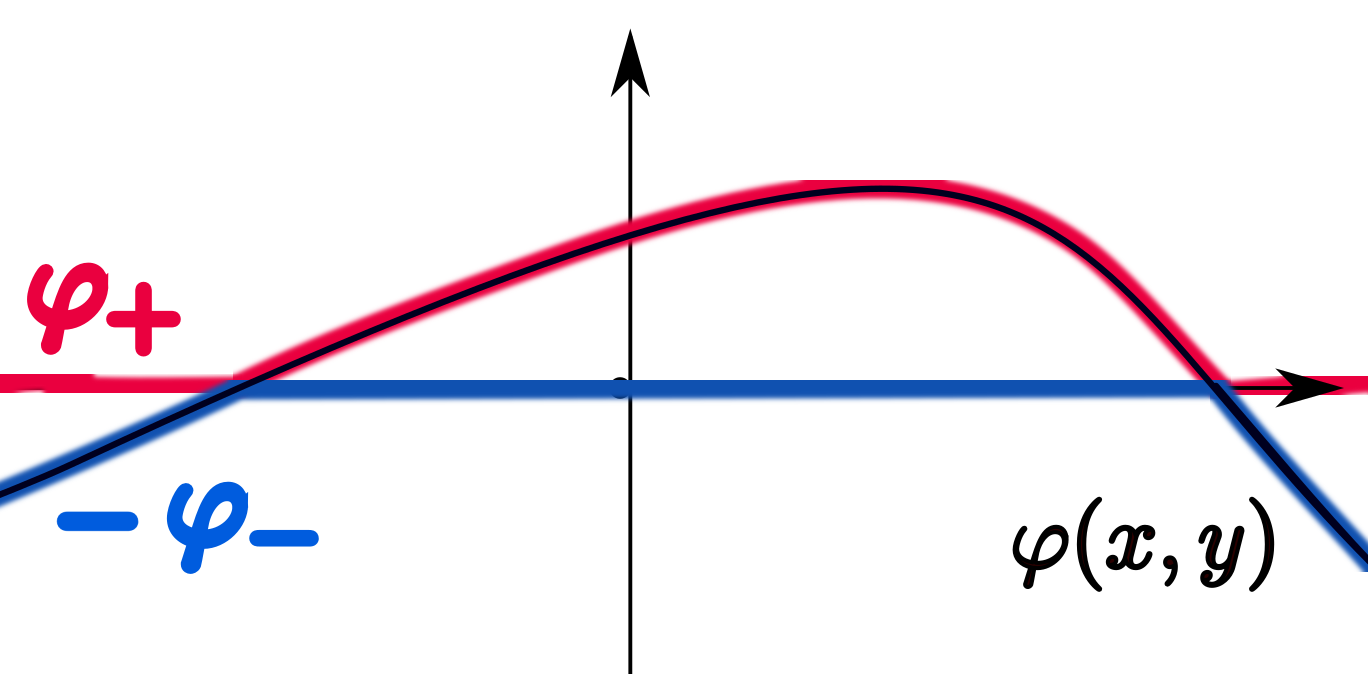
\includegraphics[scale=0.18]{assets/lectures_part_3-571a6e75.png} \end{gathered}
\qquad
\begin{gathered}
 \underbrace{ \varphi_+ + (- \varphi_- )}_{\varphi_+ - \varphi_-}= \Bigg[ \begin{gathered}
  \varphi + 0\\
  0 + \varphi
 \end{gathered} = \varphi
\end{gathered}
$$
$$
\mathbb{E} \eta = \mathbb{E} \varphi(\xi_1, \xi_2) = \mathbb{E} \left(  \varphi_+ (\xi_1, \xi_2) - \varphi_- (\xi_1, \xi_2) \right) =\mathbb{E} \varphi_+ (\xi_1, \xi_2) -  \mathbb{E} \varphi_- (\xi_1, \xi_2) \circled{=}
$$
{\small  Застосовуємо висновок про математичне сподівання невід'ємної функції:}
$$
 \circled{=} \iint\limits_{\mathbb{R}^2} \varphi_+(x,y) f_{\overline{\xi}} (x,y)dxdy - \iint\limits_{\mathbb{R}^2} \varphi_-(x,y) f_{\overline{\xi}} (x,y)dxdy =
$$
$$
= \iint\limits_{\mathbb{R}^2} \left( \varphi_+ (x,y) - \varphi_- (x,y)  \right) f_{\overline{\xi}} (x,y) dxdy =
\iint\limits_{\mathbb{R}^2} \varphi(x,y) f_{\overline{\xi}} (x,y) dxdy \quad \text{ Ч.и.т.д.}
$$

\end{proof}

\newpage

\section{Деякі додаткові ймовірнісні розподіли.}

\subsection{Гамма-розподіл.}
\subsubsection{PDF.}
Будемо називати гамма розподіленою величиною $\xi \sim \gammadistr(\alpha, \beta)\quad \alpha , \beta >0$:
$$
\begin{gathered}
f_{\xi}(x) = \begin{dcases}
     \frac{\beta^{\alpha}}{\Gamma(\alpha)} x^{\alpha-1}e^{-\beta x}, & x > 0;\\
    0, & x\leq  0;
\end{dcases}
\end{gathered} \qquad  \begin{gathered}
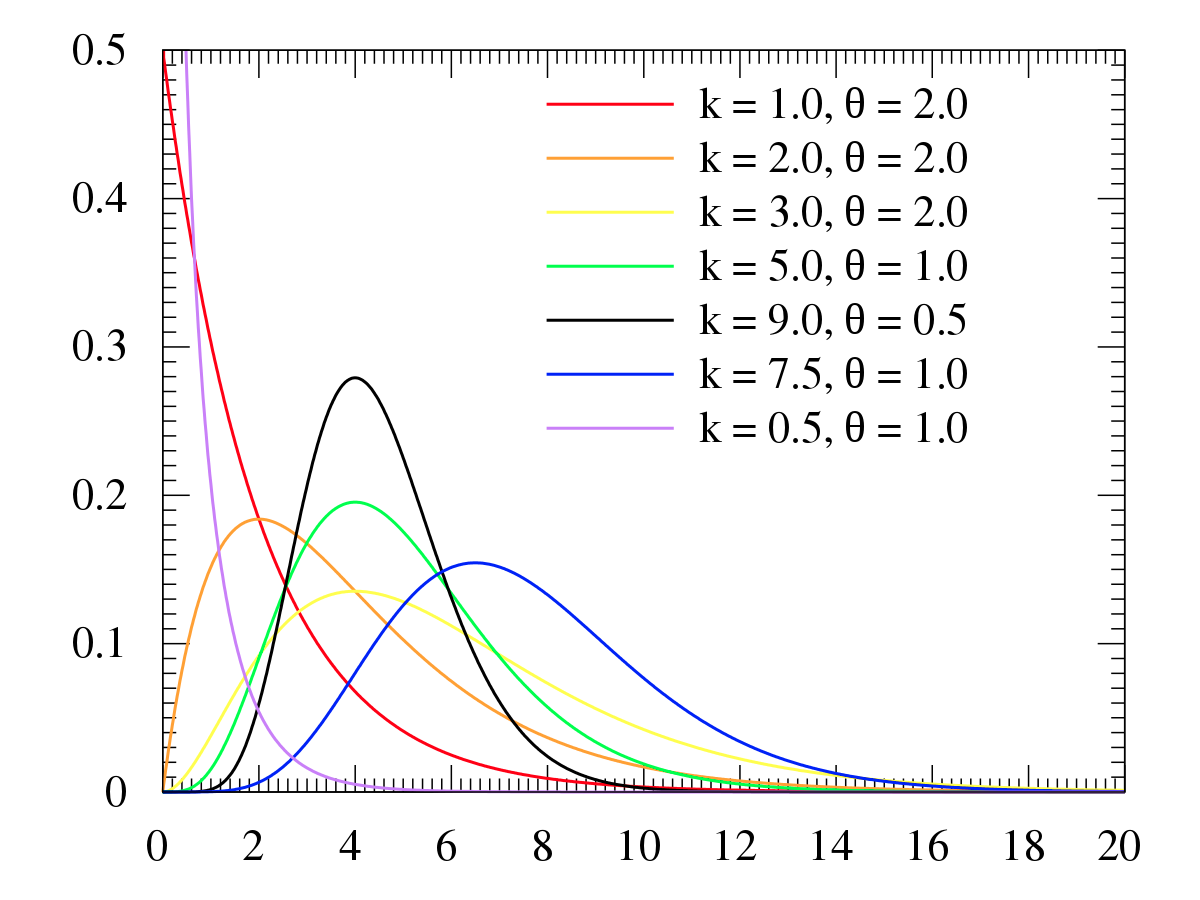
\includegraphics[scale=0.15]{assets/lectures_part_3-f657bbe5.png}
\end{gathered}
$$

За умовою нормування:
$$
1 = c  \int\limits_{9}^{ +\infty}{ x^{\alpha-1}e^{-\beta x} dx} = \frac{c}{\beta^\alpha}  \underbrace{ \int\limits_{0}^{ +\infty}{ (\beta x)^ {\alpha -1 } e^{\beta x} d (\beta x)}}_{\gammadistr{(\alpha)}}   = \frac{c \cdot \Gamma(\alpha)}{\beta^{\alpha}}  \Longrightarrow c = \frac{\beta^{\alpha}}{\Gamma(\alpha)}
$$
Розглянемо випадок $\alpha =  1$: \qquad  $f_{\Gamma(1, \beta)} (x) = \begin{dcases}
 \beta e^{-\beta x }, & x > 0 ;\\
 0, & x\leq  0 ;
\end{dcases} = f_{Exp(\beta)}$\\
Тобто, экспоненціальний розподіл є окремим випадком гамма-розподілу.
\subsubsection{Числові характеристики.}
Знайдемо одразу n-тий момент величини $ \xi \sim \Gamma(\alpha, \beta)$.
$$
\mathbb{E} \xi^n \!=\!  \!\int\limits_{0}^{ +\infty}{ x^n \cdot f_{\xi} (x) dx} \!=\! \int\limits_{0}^{ +\infty}{x^n  \frac{\beta^{\alpha}}{\Gamma(\alpha)} x^{\alpha-1}e^{-\beta x}}dx\!=\! \frac{\beta^{\alpha}}{\Gamma(\alpha)} \cdot   \int\limits_{0}^{ +\infty}{ x^{\alpha+n-1}e^{-\beta x}}dx \!=
$$
$$
=  \frac{\beta^{\alpha}}{\Gamma(\alpha) \cdot \beta^{n + \alpha}} \cdot   \int\limits_{0}^{ +\infty}{ \left( \beta x \right) ^{\alpha+n-1}e^{-\beta x}} d \left( \beta x \right)  = \fbox{$ \dfrac{\Gamma(\alpha + n)}{ \beta^n \cdot \Gamma(\alpha)}$}
$$
$
\mathbb{E} \xi = (n = 1 ) = \frac{1}{ \beta \cdot \Gamma (\alpha)} \cdot \Gamma(\alpha+1) = \frac{\alpha}{\beta}
$\\
$
\mathbb{E} \xi^2 = (n = 2) = \frac{1}{\beta^2 \cdot \Gamma (\alpha) }  \cdot \Gamma(\alpha + 2) = \frac{\alpha ( \alpha + 1)}{\beta^2}
$\\
$
\mathbb{D} \xi = \mathbb{E}(\xi^2) - \left( \mathbb{E}\xi \right) ^2 = \frac{\alpha ( \alpha + 1)}{\beta^2} - \frac{\alpha^2}{\beta^2} = \frac{\alpha}{\beta^2}
$
\subsubsection{Стійкість відносно додавання.}

Експоненціальний розподіл не є стійким відносно додавання, але більш широкий класс - гамма розподілів буде мати таку властивість.
\begin{boxteo}[Про напівстійкість Гамма-розподілу.]
$$
 \independent \begin{cases}
  \xi_1 \sim \Gamma (\alpha_1, \beta)\\
  \xi_2 \sim \Gamma (\alpha_2, \beta)
\end{cases} \quad \Longrightarrow \quad \fbox{$ \xi_1 + \xi_2 \sim \Gamma(\alpha_1 + \alpha_2 , \beta)$}
$$
\end{boxteo}

\begin{proof} За умовою, маємо:
 $$
 f_{\xi_1} = \begin{dcases}
      \frac{\beta^{\alpha_1}}{\Gamma(\alpha_1)} x^{\alpha_1-1}e^{-\beta x}, & x > 0;\\
     0, & x\leq  0;
 \end{dcases} \qquad \qquad  f_{\xi_2} = \begin{dcases}
       \frac{\beta^{\alpha_2}}{\Gamma(\alpha_2)} x^{\alpha_2-1}e^{-\beta x}, & x > 0;\\
      0, & x\leq  0;
  \end{dcases}
 $$
 $$
 \text{Скористаємося правилом згортки: }\quad f_{\xi_1 + \xi_2} (y) =  \int\limits_{-\i }^{ +\infty}{ f_{\xi_1 } (x) f_{\xi_2} (y-x) dx} =
 $$
 $$ = \textstyle{\frac{\beta^{\alpha_1}\beta^{\alpha_2}}{\Gamma{(\alpha_1)}  \Gamma(\alpha_2)} }  \displaystyle\int\limits_{0}^{y}{
 x^{\alpha_1 - 1 } e^{- \beta x} (y-x)^{\alpha_2 - 1} e^{-\beta(y-x)}dx
 }
=
 \left|
\underbrace{\begin{cases}
 x > 0 \\
 y - x > 0
\end{cases}\begin{cases}
 x > 0\\
 x < y
\end{cases}}_{x \in(0, y)}
  \right| \circled{=}
 $$
 Зауваження. Надалі будемо вважати, що при $y\leq 0 \quad f_{\xi_1 + \xi_2 } (y) =0$.
 $$
 \circled{=} \frac{\beta^{\alpha_1 + \alpha_2} e^{-\beta y}}{ \Gamma(\alpha_1) \Gamma(\alpha_2)}  \int\limits_{0}^{y}{x^{\alpha_1 - 1} (y -x)^{\alpha^2 -1 }dx} = \left| \begin{gathered}
   x = y t \quad dx = ydt\\
   x :  0 \to y \\
   t : 0 \to  1
 \end{gathered} \right|  =
 $$
 $$
 = \frac{\beta^{\alpha_1 + \alpha_2} e^{-\beta y}}{ \Gamma(\alpha_1) \Gamma(\alpha_2)}  \int\limits_{0}^{1}{ y^{\alpha_1 - 1} t^{\alpha_1 - 1} y^{\alpha_2 - 1} (1-t)^{\alpha_2 -1 }ydt } =
 $$
 $$
 =  \frac{\beta^{\alpha_1 + \alpha_2} e^{-\beta y}}{ \Gamma(\alpha_1) \Gamma(\alpha_2)} \cdot y^{\alpha_1 + \alpha_2 - 1} \cdot \underbrace{\int\limits_{0}^{1}{t^{\alpha_1 - 1} (1 - t )^{\alpha_2 -1} dt} }_{\beta(\alpha_1 , \alpha_2)= \frac{\Gamma(\alpha_1)\Gamma(\alpha_2)}{\Gamma(\alpha_1+ \alpha_2)} }= \frac{\beta^{\alpha_1 + \alpha_2} e^{-\beta y}}{ \Gamma(\alpha_1 + \alpha_2)} \cdot y^{\alpha_1 + \alpha_2 - 1} =
 $$
 $$
 = \begin{dcases}
   \frac{\beta^{\alpha_1 + \alpha_2}}{ \Gamma(\alpha_1 + \alpha_2)} \cdot y^{\alpha_1 + \alpha_2 - 1} e^{-\beta y}, & y > 0;\\
   0 & y \leq 0;
 \end{dcases} = f_{\Gamma(\alpha_1 + \alpha_2 , \beta)} (y)
 $$
\end{proof}

\subsection{Chi-square distribution with n degrees of freedom.}
\subsubsection{PDF.}
Розглядаємо $\xi_1 ,..., \xi_n $ - незалежні гаусівські $N(0,1)$. Інакше: $ \overline{\xi} = \begin{bmatrix}
 \xi_1 \\
 \vdots\\
 \xi_n
\end{bmatrix} \sim N(\vec{0}, I)$.
Розподіл $ \chi^2_n $ - це закон розподілу $ \left| \left| \overline{\xi} \right|  \right|^2 =  \sum\limits_{i = 1}^{n}{\xi_i^2}$.\\
$
n = 1.$ Шукаємо: $  \xi^2, \xi \sim N(0,1)$.
$$
\varphi(x)  = x^2 \quad x^2 = y \Longrightarrow x = \pm \sqrt{y} \Longrightarrow \begin{gathered}
\psi_1(y) = - \sqrt{y}\\
\psi_2 (y) = \sqrt{y}
\end{gathered} \quad E_{\varphi_1} = \mathbb{E}_{\varphi_2} = [0, + \infty]
$$
$$
f_{\varphi(\xi)} (y) =  \sum\limits_{i = 1}^{2}{ f_{\xi}} \left( \psi_i (y) \right)  \cdot \left| \psi'_i(y) \right| \cdot \index{}\left\lbrace y \in E_{\varphi_i} \right\rbrace
 =
 $$
 $$
 = \frac{1}{ \sqrt{2 \pi} } e^{- \frac{x^2}{2} } \bigg|_{x = -\sqrt{y}} \cdot \left| \left( - \sqrt{y} \right)'  \right| \cdot \index{R_+} (y)  +  \frac{1}{ \sqrt{2 \pi} } e^{- \frac{x^2}{2} } \bigg|_{x = \sqrt{y}} \cdot \left| \left( \sqrt{y} \right)'  \right| \cdot \index{R_+} (y) =
 $$
 $$
 = \frac{2}{ \sqrt{2 \pi} } e^{- \frac{y}{2} } \cdot \frac{1}{ 2 \sqrt{y}} \cdot \index{R_+} (y) = \begin{cases}
  \frac{1}{\sqrt{2\pi}} y^{- \frac{1}{2} } \cdot e^{ - \frac{1}{2}y}, & y > 0; \\
  0 , & y \leq  0
 \end{cases}   = f_{ \chi_1 ^2} (y)
 $$
$n \in \mathbb{N}.$ Шукаємо: $ \sum\limits_{i = 1}^{n}{\xi_i^2}  \quad \forall \xi_i  : \xi_i \sim N(0,1)$.\\
Розглянемо щільність $ f_{ \chi_1 ^2} (y)$:
$$
\begin{dcases}
\frac{1}{\sqrt{2\pi}} y^{- \frac{1}{2} } \cdot e^{ - \frac{1}{2}y}, & y > 0; \\
0 , & y \leq  0
\end{dcases} =
\begin{dcases}
 \frac{\left( \frac{1}{2} \right) ^{ 1/2 }}{\Gamma \left(  \frac{1}{2}  \right) }  y^{ \frac{1}{2}  - 1} e^{ - \frac{1}{2} y } , & y > 0; \\
 0 , & y \leq  0
\end{dcases} \quad \begin{gathered}
 \text{Впізнаємо гамма-розподіл:}\\
 \chi_1^2 \sim \Gamma \left( \frac{1}{2} ; \frac{1}{2}  \right)
\end{gathered}
$$
Тоді, $\chi^2_n$ це сумма n-незалежних $\chi_1^2$: $\chi^2_n = \underbrace{\chi_1^2 + ... + \chi_1^2}_{n} = \Gamma \left(  \frac{n}{2}, \frac{1}{2} \right)  $
$$
f_{
\chi_n^2
} (x) = \begin{dcases}
 \frac{ \frac{1}{2}^{ \frac{n}{2}  }  }{ \Gamma \left(  \frac{n}{2}  \right) } x^{ \frac{n}{2} -1  } e^{- \frac{1}{2}x }, & x > 0;\\
 0 , & x \leq 0;
\end{dcases}  =
\begin{dcases}
\frac{ 1 }{2^{ \frac{n}{2}  }  \Gamma \left(  \frac{n}{2}  \right) } x^{ \frac{n}{2} -1  } e^{- \frac{x}{2} }, & x > 0;\\
0 , & x \leq 0;
\end{dcases}
$$
$n = 2.$ Зокрема, в такому випадку, отримаємо: $ \chi_2^2 = \Gamma \left( 1, \frac{1}{2}  \right) = Exp \left( \frac{1}{2} \right)  $.
\begin{center}
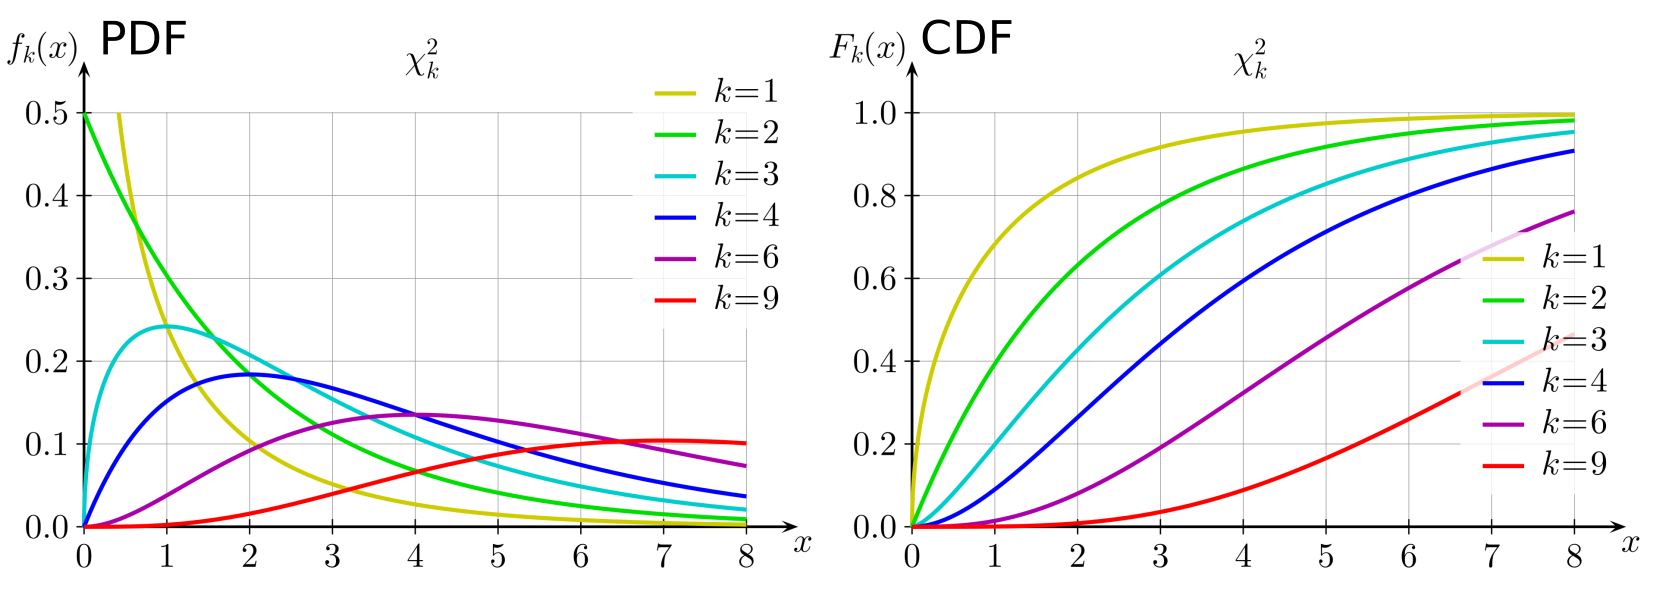
\includegraphics[scale=0.3]{assets/lectures_part_3-d1334d87.png}
\end{center}
\subsubsection{Числові характеристики.}
$\mathbb{E} \chi^2_n = \mathbb{E} \Gamma \left( \frac{1}{2} , \frac{1}{2}   \right) = n  \quad \left[ \mathbb{E} \left( \xi_1^2 + ... \xi_n^2 \right) = \mathbb{E} \xi_1^2 + ... + \mathbb{E}\xi_n^2 = n \right]$\\
$\mathbb{D} \chi^2_n = \mathbb{D} \Gamma \left( \frac{1}{2} , \frac{1}{2}   \right) = 2n $

\subsection{t-розподіл Стьюдента з n степенями вільності.}
\begin{wrapfigure}{R}{0.48\textwidth}
\centering
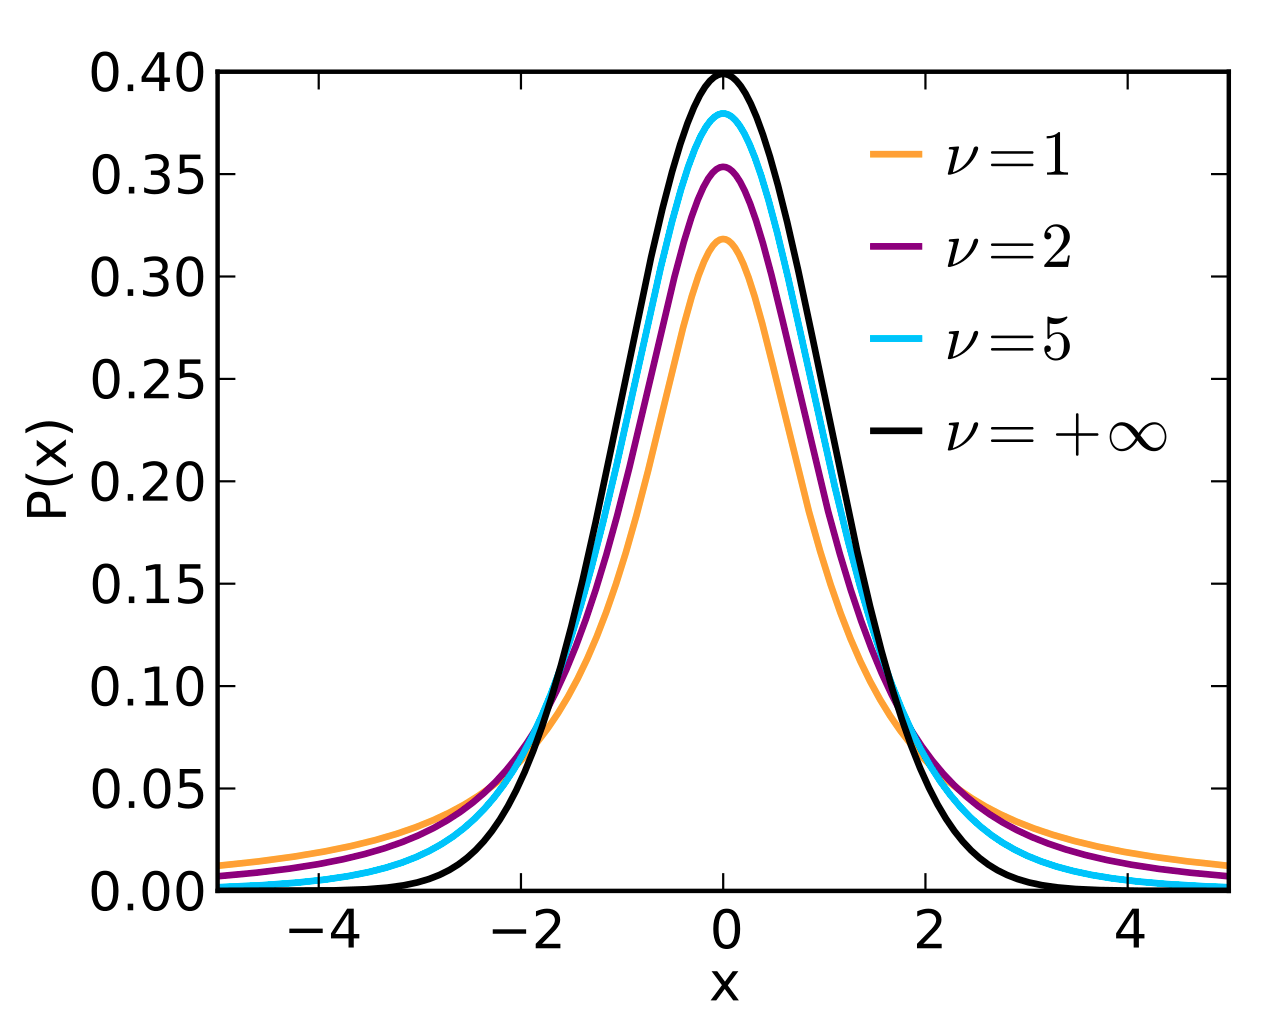
\includegraphics[width=0.45\textwidth]{assets/lectures_part_3-91d0349d.png}
The PDF of the Student distribution.
\end{wrapfigure}
Позначається $t_n $ або $ St_n$. Розглядаємо розподіл такої величини $\eta$:
$$\eta = \frac{\xi_0}{\sqrt{ \frac{\xi_1^2 + ... + \xi_n^2}{n} }} = \xi_0 \frac{n}{ \sqrt{
\chi^2_n
}} ,$$
де $\xi_0, \xi_1, ... , \xi_n - $ незалежні стандартні гаусівські величини.
$$
\begin{gathered}
f_{St_n}(x) = \frac{\Gamma(\frac{n+1}{2})} {\sqrt{n\pi}\,\Gamma(\frac{n}{2})} \left(1+\frac{x^2}{n} \right)^{\!-\frac{n+1}{2}}
\end{gathered}
% \qquad
% \begin{gathered}
%   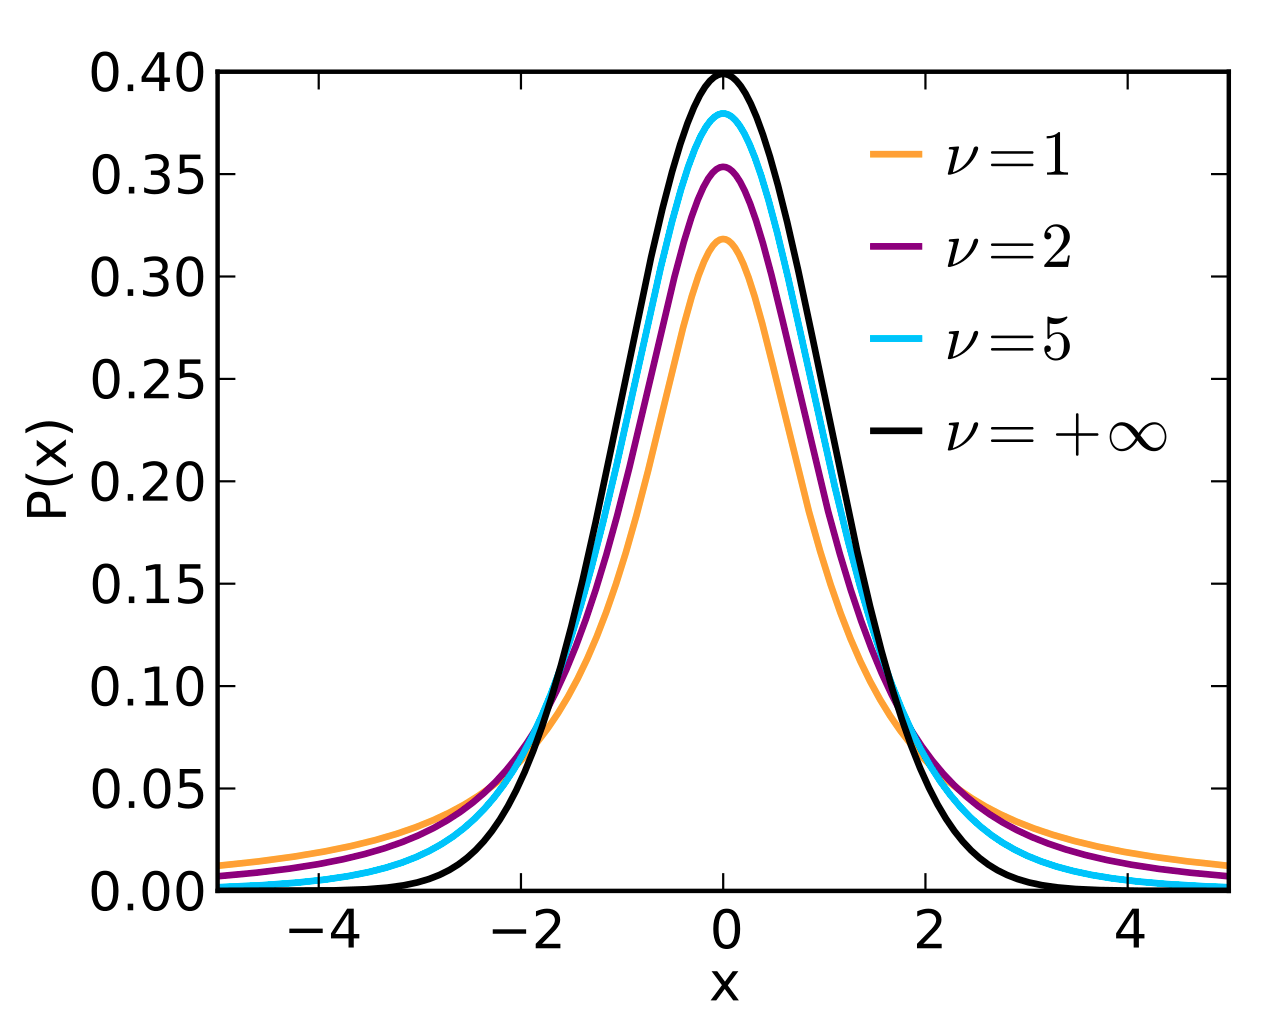
\includegraphics[scale=0.14]{assets/lectures_part_3-91d0349d.png}
% \end{gathered}
$$

$а$\\
\par
$а$\\
\par
Слід зауважити, що у випадку $n = 1 : St_1$ отримаємо розподіл Коші:
$$
f_{St_1} (x) = \frac{1}{ \pi ( 1 + x^2)}
$$
Якщо спрямуємо $n \to \infty$, отримаємо стандартний гаусівський розподіл:
$$
f_{St_\i} = \frac{1}{\sqrt{2 \pi}} e^{- \frac{t^2}{2} }
$$



\subsection{Розподіл Фішера(-Снедекора)}
\begin{wrapfigure}{R}{0.48\textwidth}
\centering
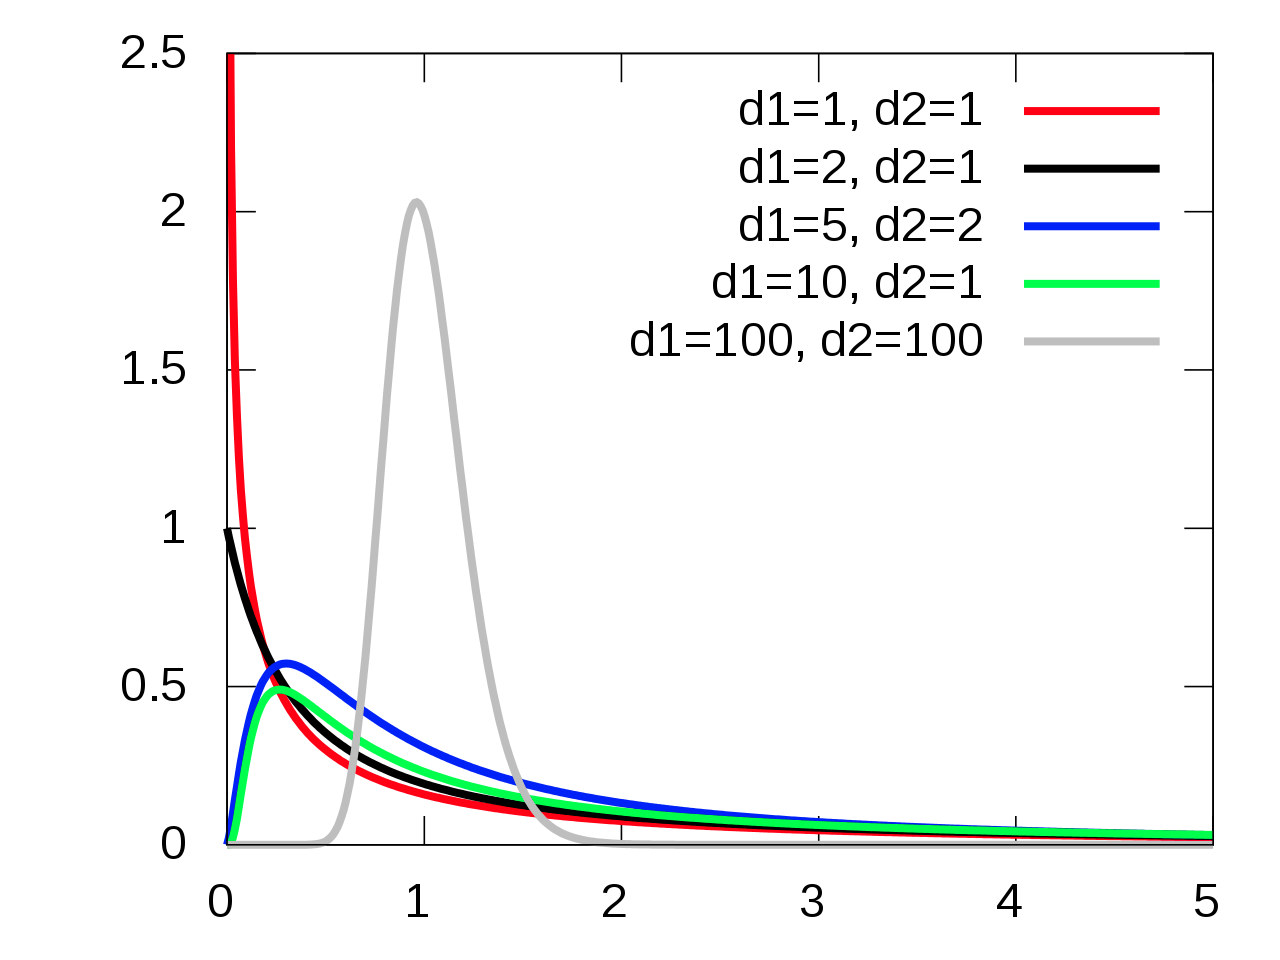
\includegraphics[width=0.45\textwidth]{assets/lectures_part_3-c1782fcb.png}
The PDF of the F-distribution
\end{wrapfigure}
Позначається $F_{m,n}$. Розглядаємо розподіл такої величини $\omega:$
$$
\omega = \frac{\left( \xi_1^2 + ... + \xi_m^2 \right)/ m }{\left( \eta_1^2 + ... + \eta_n^2 \right)/n}
$$
де $\xi_0, \xi_1, ... , \xi_m, \eta_1, ... , \eta_n - $ незалежні стандартні гаусівські величини.
$$
f(x; d_1,d_2) = \frac{\sqrt{\frac{(d_1x)^{d_1}d_2^{d_2}} {(d_1x+d_2)^{d_1+d_2}}}} {x\beta\!\left(\frac{d_1}{2},\frac{d_2}{2}\right)}
$$
$ф$\\
\par
$ф$\\
\par

\newpage

\section{Граничні теореми теорії ймовірностей}

\subsection{Нерівність Чебишова.}
$\xi$ - випадкова величина, для якої $\exists \mathbb{E}\xi \  \exists \mathbb{D} \xi$.\\
\par
Знаємо, що $
\mathbb{D} \xi = \mathbb{E} (\xi - \mathbb{E} \xi)^2
$. Але дисперсія є більше теоретичною величиною. Наприклад, розглянемо прилад, який перестає працювати якщо напруга в мережі $\xi = U_{\text{м}} $ відхиляється $\xi < 180 $ або $ \xi > 260$.\\
Інакше кажучи, якщо $ \left| \xi - \mathbb{E}\xi \right| > 40$ - прилад не працює. Нас цікавить ймовірність $\mathbb{P} \left\lbrace \left| \xi - \mathbb{E} \xi \right| > a \right\rbrace \!\!= ?$. Але, знаючи дисперсію, не зрозуміло, як пов'язати цю характеристику з ймовірністю зазначеної критичної події. \\Саме таку оцінку дає нерівність Чебишова.
\begin{boxteo}[нерівність Чебишова]
Якщо $\exists \mathbb{D} \xi$, то:
$$
\forall a > 0 \quad \mathbb{P} \left\lbrace \left| \xi - \mathbb{E} \xi \right| \geq a \right\rbrace \leq \frac{\mathbb{D} \xi}{a^2}
$$
Перевага: Обчислюється лише через дисперсію. Не залежить від розподілу.\\
Недолік: нерівнісь дає дуже грубу оцінку ймовірності.
\end{boxteo}
\begin{consequence}
    $$\mathbb{P} \left\lbrace \left| \xi - \mathbb{E} \xi \right| < a \right\rbrace = \mathbb{P} \left\lbrace  \xi \in \left(  \mathbb{E}  \xi - a, \mathbb{E}\xi + a \right) \right\rbrace \geq  1 - \frac{ \mathbb{D} \xi}{a^2 } $$
\end{consequence}
\textbf{Лема. }(нерівність Маркова)
$\eta$ - невід'ємна випадкова величина $\mathbb{P} \left\lbrace \eta \geq 0 \right\rbrace = 1$.
\\Тоді:\ \fbox{$ \mathbb{P} \left\lbrace  \eta \geq a \right\rbrace \leq  \dfrac{\mathbb{E} \eta}{a} $}
\begin{proof}
$$
\mathbb{E} \eta = \mathbb{E} \left( \eta \cdot \index{} \left\lbrace 0 \leq \eta < a \right\rbrace
+ \eta\cdot \index{} \left\lbrace  \eta \geq a\right\rbrace
 \right) = \mathbb{E} \eta \cdot  \index \left\lbrace \eta < a \right\rbrace + \mathbb{E} \eta\cdot \index \left\lbrace   \eta \geq  a \right\rbrace \geq
$$
$$
\geq  \mathbb{E} \eta \cdot \index \left\lbrace \eta \geq a  \right\rbrace \geq  \mathbb{E} a \cdot \index \left\lbrace  \eta \geq a \right\rbrace = a \cdot \mathbb{E} \index \left\lbrace \eta \geq a  \right\rbrace = a \cdot \mathbb{P} \left\lbrace \eta \geq a \right\rbrace
$$

\end{proof}

\begin{proof}(До нерівності Чебишова.) Очевидно, що:
$$
\eta = \left( \xi - \mathbb{E} \xi \right)^2 \geq 0
$$
 За нерівністю Маркова:
 $$
  \mathbb{P} \left\lbrace \left| \xi - \mathbb{E} \xi \right| \geq a  \right\rbrace=\mathbb{P} \left\lbrace  (\xi - \mathbb{E} \xi)^2 \geq a^2 \right\rbrace \leq \frac{\mathbb{E} \left( \xi - \mathbb{E} \xi \right)^2}{a^2} = \frac{\mathbb{D}\xi}{a^2}
 $$
\end{proof}
\newpage
\subsection{Види збіжності випадкових величин}
З мат. аналізу пам'ятаємо означення збіжності числової послідовності:
\begin{defo} (Нагадування) \\
 Послідовність $ \left\lbrace x_n\ \Big|\  n\in \mathbb{N} \right\rbrace$ збігається до $x$ якщо:
 $$
 \forall \varepsilon >0 \ \exists N \ \forall n\geq N \ |x_n - x| < \varepsilon
 $$
Для $(\xi_n)$ - послідовності випадкових величин, єдиного аналогічного означення не існує. Тому, доведеться розглянути декілька видів видів збіжності.
\end{defo}
\subsubsection{Збіжність з імовірністю 1.}
Позначення: \fbox{\textbf{м.н.}-збіжність.}
\begin{defo} Нехай задана послідовність $(\xi_n) = \left\lbrace \xi_n \Big| n \in \mathbb{N} \right\rbrace$, тоді:
 $$
 (\xi_n) \xrightarrow[n \to \infty]{\text{м.н.}} \xi \Longleftrightarrow \mathbb{P} \left\lbrace \xi_n \to \xi \right\rbrace = 1 \Longleftrightarrow \mathbb{P} \left\lbrace \omega : \xi_n (\omega) \to \xi(\omega) \right\rbrace = 1
 $$
 називається збіжністю з імовірністю 1 або м.н. збіжністю.
 \begin{enumerate}
     \item Найбільш природній вид збіжності.
     \item Досить незручний для використання.
 \end{enumerate}
\end{defo}
\subsubsection{Збіжність в середньому квадратичному.}
Позначення: \fbox{$\mathbb{L}_2$-збіжність.}
\begin{defo} Нехай задана послідовність $(\xi_n) = \left\lbrace \xi_n \bdash n \in \mathbb{N} \right\rbrace$, тоді:
  $$
  (\xi_n) \xrightarrow[n \to \infty]{\mathbb{L}_2}\xi \Longleftrightarrow \mathbb{E} \left( \xi_n - \xi \right)^2 \xrightarrow[n \to \infty]{} 0
  $$
  називається збіжністю в середньому квадратичному.
\end{defo}
\subsubsection{Збіжність в середньому.}
Позначення: \fbox{$\mathbb{L}_1$-збіжність.}
\begin{defo} Нехай задана послідовність $(\xi_n) = \left\lbrace \xi_n \bdash n \in \mathbb{N} \right\rbrace$, тоді:
  $$
  (\xi_n) \xrightarrow[n \to \infty]{\mathbb{L}_2}\xi \Longleftrightarrow \mathbb{E} \left| \xi_n - \xi \right| \xrightarrow[n \to \infty]{} 0
  $$
  називається збіжністю в середньому.
\end{defo}
\subsubsection{Збіжність за імовірністю.}
Позначення: \fbox{$\mathbb{P}$-збіжність.}\\
Надалі \textbf{критичною подією} будемо називати велике відхилення однієї величини від іншої на фіксоване додатнє число, тобто: $\varepsilon  > 0 : \left| \xi_n - \xi \right| > \varepsilon $.
\begin{defo} Нехай задана послідовність $(\xi_n) = \left\lbrace \xi_n \bdash n \in \mathbb{N} \right\rbrace$, тоді:
  $$
  (\xi_n) \xrightarrow[n \to \infty]{\mathbb{P}}\xi \Longleftrightarrow
  \forall \varepsilon > 0 \ \
\mathbb{P} \left\lbrace   \left| \xi_n - \xi \right| > \varepsilon  \right\rbrace \xrightarrow[n\to\infty]{}0
  $$
  називається збіжністю за імовірністю.
\end{defo}
\begin{remark} Для збіжності за імовірністю справедливою є еквівалентність:
$$
\left( \forall \varepsilon > 0 \ \
\mathbb{P} \left\lbrace   \left| \xi_n - \xi \right| > \varepsilon  \right\rbrace \xrightarrow[n\to\infty]{}0 \right) \Longleftrightarrow \left( \forall \varepsilon  > 0 \ \
\mathbb{P} \left\lbrace   \left| \xi_n - \xi \right| \leq  \varepsilon  \right\rbrace \xrightarrow[n\to\infty]{}1 \right)
$$
\end{remark}
\begin{wrapfigure}{R}{0.4\textwidth}
\centering
\vspace*{-1.5cm}
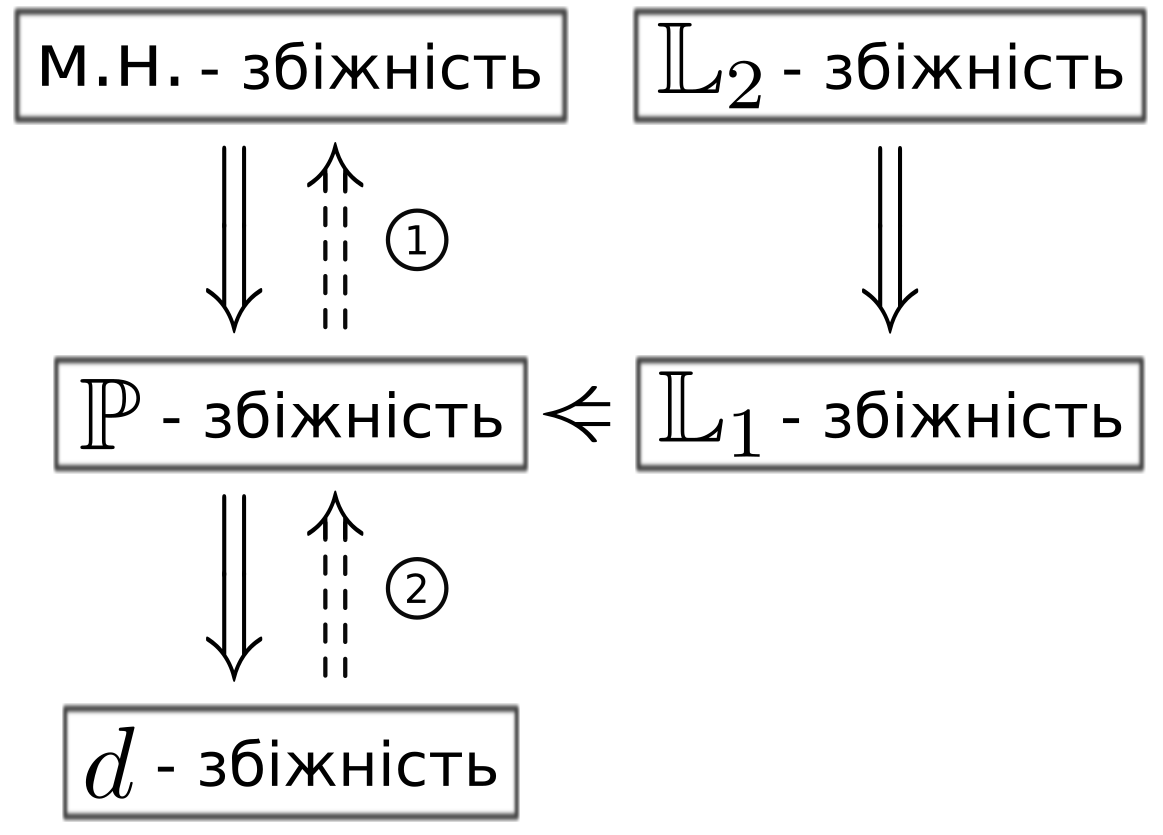
\includegraphics[width=0.39\textwidth]{assets/g11500.png}
{\small Cхема зв'язку різних видів збіжності.}
\end{wrapfigure}
\subsubsection{Взаємозв'язок збіжностей.}
 Кожна стрілки відповідає теоремі, що описує зв'язок збіжностей.\\
 Пунктирні стрілки 1 та 2 потребують додаткового пояснення:\\
    $\circled{1}$. Завжди існує м.н.-збіжна підпослідовність.\\
    $\circled{2}$. Виконується, якщо $\xi = const$.
\\
\def\L{\mathbb{L}}

\textbf{Лема.} (Нерівність Ляпунова (ч.в.)) $$\mathbb{E} \left| \eta \right| \leq \sqrt{\mathbb{E} \eta^2} $$
\begin{proof}
 $\mathbb{E} ( \left|\eta \right|^2 ) - \left( \mathbb{E} \left| \eta \right| \right)^2=  \mathbb{E} (\eta^2) - (\mathbb{E} \left| \eta \right|)^2=  \mathbb{D} \left| \eta \right| \geq  0 \Rightarrow  \mathbb{E} \left| \eta \right| \leq \sqrt{\mathbb{E} \eta^2} $
\end{proof}
\begin{teo} Покажемо, що $\L_2 \Longrightarrow \L_1$, тобто:
$$
 \begin{gathered}
  \L_2 : \mathbb{E} (\xi_n - \xi)^2 \xrightarrow[n\to\i]{} 0\\
  \Downarrow\\
  \L_1 : \mathbb{E} \left| \xi_n - \xi \right| \xrightarrow[n\to\i]{} 0\\
 \end{gathered}
$$
\end{teo}
\begin{proof}За нерівністю Ляпунова та правилом ''2-ох міліціонерів'':
$$
0 \leq  \underbrace{\mathbb{E} \left|  \xi_n - \xi \right|}_{\to 0} \leq  \sqrt{\mathbb{E}(\xi_n - \xi)^2} \xrightarrow[n\to\infty]{} 0\  \Longleftarrow\   \L_2\text{-збіжність.}
$$
\end{proof}
\begin{teo} Покажемо, що $\L_1 \Longrightarrow \mathbb{P}$, тобто:
$$
 \begin{gathered}
 \L_1 : \mathbb{E} \left| \xi_n - \xi \right| \xrightarrow[n\to\i]{} 0\\
  \Downarrow\\
\mathbb{P}: \ \ \forall \varepsilon > 0 : \mathbb{P} \left\lbrace \left| \xi_n - \xi \right| > \varepsilon \right\rbrace \xrightarrow[n\to\i]{} 0\\
 \end{gathered}
$$
\end{teo}
\begin{proof} Підставимо $ \left| \xi_n  - \xi\right|$ у нерівність Маркова:
$$
0  \leq \underbrace{\mathbb{P} \left\lbrace \left| \xi_n  - \xi\right| > \varepsilon  \right\rbrace}_{\to 0} \leq \frac{\mathbb{E} \left| \xi_n  - \xi\right|}{\varepsilon } \xrightarrow[n\to\i]{} 0 \  \Longleftarrow\   \L_1\text{-збіжність.}
$$
За правилом  ''2-ох міліціонерів'' отримали збіжність імовірності до 0.
\end{proof}

\subsubsection{Збіжність за розподілом (слабка збіжність).}

Позначення: \fbox{\textbf{d}-збіжність.}
\begin{defo} Нехай задана послідовність $(\xi_n) = \left\lbrace \xi_n \Big| n \in \mathbb{N} \right\rbrace$, тоді:
 $$
 (\xi_n) \xrightarrow[n \to \infty]{d} \xi \Longleftrightarrow\  \begin{gathered}
  F_{\xi}(x)\in C^{1}(D)\\
  F_{\xi_n}(x)\in C^{1}(D)
 \end{gathered}\ \  \forall x \in D:  \underbrace{F_{\xi_n}(x)}_{\mathbb{P} \left\lbrace \xi_n < x \right\rbrace} \xrightarrow[n\to\i]{} \underbrace{F_{\xi}(x)}_{\mathbb{P} \left\lbrace \xi< x \right\rbrace}
 $$
 називається збіжністю за розподілом.\\
\end{defo}
\begin{teo} Покажемо, що $d \Longrightarrow \mathbb{P}$ якщо $ \xi = const$, тобто:
$$
 \begin{gathered}
 d : \ \ \exists C \in \mathbb{R} \  \ \forall x \neq C:  F_{\xi_n}(x) \xrightarrow[n\to\i]{}F_{C}(x) \\
  \Downarrow\\
\mathbb{P}: \ \ \forall \varepsilon > 0 : \mathbb{P} \left\lbrace \left| \xi_n - C \right| > \varepsilon \right\rbrace \xrightarrow[n\to\i]{} 0\\
 \end{gathered}
$$
\end{teo}
\begin{proof} Умову збіжності послідовності $(\xi_n)$ за розподілом до константи $\exists C \in \mathbb{R}$ природнім чином можна представити як:
$$
(\xi_n) \xrightarrow[n\to\infty]{} C \ \Longleftrightarrow \ \mathbb{P} \left\lbrace \xi_n < x  \right\rbrace \xrightarrow[n\to\infty]{}
\begin{cases}
 0 ,& x \leq  C; \\
 1 ,&  x > C ;
\end{cases} = F_C(x)
$$
В той же час, умову збіжності за імовірністю можна розписати так:
$$
(\xi_n) \xrightarrow[n \to \infty]{\mathbb{P}} C \Longleftrightarrow
\forall \varepsilon > 0 \ \
\mathbb{P} \left\lbrace   \xi_n \in [C - \varepsilon, C + \varepsilon]   \right\rbrace \xrightarrow[n\to\infty]{}1
$$
Розпишемо, скориставшись правилом $\mathbb{P} \left\lbrace  \xi \in [a,b) \right\rbrace = F_{\xi}(b) - F_{\xi}(a)$:
$$
1 \geq \mathbb{P} \left\lbrace \xi_n \in [C - \varepsilon , C + \varepsilon ] \right\rbrace \geq \mathbb{P} \left\lbrace \xi \in [C- \varepsilon, C + \varepsilon ] \right\rbrace =
$$
$$
= F_{\xi_n} (C+ \varepsilon )- F_{\xi_n} (C - \varepsilon ) \xrightarrow[n\to\infty]{} F_C(C + \varepsilon) - F_C(C - \varepsilon ) = 1 - 0 = 1
$$
Тому, за правилом ''2-ох міліціонерів'', отримали збіжність послідовності $(\xi_n)$ за імовірністью до константи $C$. Отже: $ d \xRightarrow[]{\xi=const} \mathbb{P} $.
\end{proof}
\begin{remark}
    Для всіх видів збіжності виконуються арифм. власт. границь.
\end{remark}
\subsubsection{Критерій середньоквадратичної збіжності до константи.}
\begin{boxteo} Нехай задана послідовність $(\xi_n) = \left\lbrace \xi_n \Big| n \in \mathbb{N} \right\rbrace$, тоді:
  $$
  \exists C \in \mathbb{R} : (\xi_n) \xrightarrow[]{\L_2} C \ \Longleftrightarrow \  \begin{cases}
   \mathbb{E} \xi_n \xrightarrow[n\to\infty]{} C; \\
   \mathbb{D} \xi_n \xrightarrow[n\to\infty]{} 0;
  \end{cases}
  $$
\end{boxteo}
\begin{proof}
 $$
 (\xi_n) \xrightarrow{ \L_2 } C \Longleftrightarrow  \mathbb{E} (\xi_n - C)^2  \xrightarrow[n\to\infty]{} 0 \Longleftrightarrow \mathbb{E} \left( \left( \xi_n  - \mathbb{E} \xi_n \right) + (\mathbb{E} \xi_n - C) \right)^2 \xrightarrow[n\to\infty]{} 0  \Longleftrightarrow
 $$
 $$
 \Longleftrightarrow \mathbb{E} (\xi_n - \mathbb{E} \xi_n)^2 + \mathbb{E}\left(  (\mathbb{E}\xi_n - C)^2 \right) + 2 \mathbb{E}(\xi_n - \mathbb{E}\xi_n) (\mathbb{E}\xi_n - C) \xrightarrow[n\to\infty]{} 0  \Longleftrightarrow
 $$
 $$
  \Longleftrightarrow \mathbb{D} \xi_n + ( \mathbb{E}\xi_n - C)  \xrightarrow[n\to\infty]{} 0 \Longleftrightarrow \begin{cases}
   \mathbb{E} \xi_n \xrightarrow[n\to\infty]{} C; \\
   \mathbb{D} \xi_n \xrightarrow[n\to\infty]{} 0;
  \end{cases}
  $$
\end{proof}

\begin{boxteo}[Окремий випадок теореми неперервності П.Леві]
$$
(\xi_n) \xrightarrow{d} \xi \ \Longleftrightarrow \ \forall t \in \mathbb{R} \ \  \underbrace{\chi_{\xi_n}}_{\mathbb{E} e ^{it \xi_n}} (t) \xrightarrow[n\to\infty]{}  \underbrace{\chi_{\xi}(t)}_{\mathbb{E} e ^{it \xi_n}}
$$
Без доведення. \ \ $\blacksquare$
\end{boxteo}


\end{document}
